%!TEX root =  main.tex
\chapter{Micro clouds}\label{chapter:Micro_clouds}
%
In this section, the core idea of this thesis will be presented. We will introduce the model of distributed \textbf{$\upmu$Cs} and show how such a system could be dynamically formed and formally described. The \textbf{$\upmu$Cs} is based on the traditional CC organizational model but adapted for different environments, allowing the creation of distributed clouds.

Throughout this section, we are going to rely on the research presented in Chapters~\ref{chapter:Intro} and~\ref{chapter:Review}, and make a connection with the existing CC model.

In Section~\ref{sec:configurable_model_structure} we present a high overview of the system -- an architecture that is influenced by the standard CC model but adapted for a different environment. Section~\ref{sec:separation_of_concerns} introduces the separation of concerns model for previously defined system architecture. Section~\ref{sec:application_model} presents a possible application model and how users can utilize newly created architecture fully. Application models are based on existing development models, so that transition is fairly easy. Possibilities how this system could be offered as a service, and which options can be offered to the potential users for developing their applications is discussed in Section~\ref{sec:as_a_service_model}. Section~\ref{sec:immutable_infrastructure} presents the desired option for infrastructure and application deployment, and discusses why immutability is important in a $\upmu$C geo-distributed environment. Section~\ref{sec:formal_model} discusses the importance of formal models in computer science, and DS in particular. This Section also presents formal models for all protocols used for the proper system formation and operation. Section~\ref{sec:long_live_transactions} shows transactions that appear in such complex system, and garbage collection done on resources that are not used anymore. Section~\ref{sec:system_observability} shows system observability mechanisms important for geo-distributed environments like $\upmu$Cs. Section~\ref{sec:access_pattern} shows access patterns that could be used in $\upmu$Cs and geo-distributed environments. 
Section~\ref{sec:Auto Scaling} presents the possibility how micro clouds could be scaled automaticaly, while Section~\ref{sec:user_data} presents flow of user data in micro clouds model. This chapter is concluded with Section~\ref{sec:repercussion} which presents repercussion of the proposed model, and how it can be used as a stand-alone model where other features could be implemented on top of that or used as service for other, existing, systems.
%
%
\section{Configurable Model Structure}\label{sec:configurable_model_structure}
%
In their work~\cite{SatyanarayananK19} Satyanarayanan et al. propose a new architecture pattern and separation into the three tiers, where every tier or layer has a distinct role. This idea is a very powerful one because applications can now be split into parts and optimized for the specific role in the global picture. On the other hand, too many moving parts mean more problems, and the whole system is potentially more prone to errors and failures.

If the previous model is taken and combined with $\upmu$DCs and a zonally based server organization, a good starting point for building $\upmu$C infrastructure, and EC as a service is achieved. This extension is an interesting move because the computing power and storage capacity that serves the nearby population can then be extended. This base model is just a starting point that is promising, but to make a fully functional model, it needs to be made more available and resilient with less latency. To achieve such behavior, these concepts have to be extended and adapted for different usage scenarios, but a geo-distributed idea from our vision should not be lost.

To extend the system in a new direction, we can look for some inspiration in existing systems that are proven and working. This is especially important in DS, so we want to lower down the complexity and avoid known problems by sticking to existing models and algorithms. When the CC design is observed, it can be seen that every single part in that system contributes to a more resilient and scalable system. On the high level, the CC architecture is separated into few building blocks that make the whole system lot easier to understand, maintain and operate.

The first building block of CC architecture is a cluster, and a cluster can be defined as a set of nodes or servers that operate as a single unit to achieve some goal. This is where resources are, and this is where user applications are running on. The next building block that consists of multiple clusters is called Regions (or DCs). Regions are isolated and independent from each other, and they contain resource application needs. These resources come in form of clusters. Regions are usually composed of a few availability zones~\cite{SouzaMFAK19}. These zones are the defense against the fail. If for whatever reason, one zone fails or goes offline, there are still more of them to serve user requests, there is a better availability, scalability, and resilience.

If we now observe $\upmu$Cs as geo-distributed systems with dispersed users~\cite{hal-01067888}, we can use a similar model with some adaptations. Rely on a similar proven strategy, do not build the entire model, but adapt the existing one for the different use-case.

Table~\ref{tab:table5} presents similar concepts between CC and edge-centric computing (ECC) concepts. The accent is here put on the difference between the physical logical concepts in the two models.

\begin{table}[h!]
	\begin{center}
		\begin{tabular}{l|l}
			\textbf{Edge centric computing} & \textbf{Cloud computing}\\
			\hline
			Topology (logical) & Cloud provider (logical)\\
			Region (logical) & Region (physical)\\
			Cluster (physical) & Zone (physical)\\
		\end{tabular}
	\end{center}
	\vspace{-0.5cm}
	\caption{Similar concepts between cloud computing and ECC.}
	\label{tab:table5}
\end{table}

\noindent
Since we are talking about geo-distributed systems, our scenario is a little bit different than the one used in the standard CC model. We can still combine multiple EC nodes into clusters, that is what $\upmu$DCs already propose. If we want to go a little bit further, we can define a cluster as a:

\begin{definition}
	A $\upmu$C cluster is a group of nodes that are virtually and/or geographically separated, that works together to provide the same service to clients.
\end{definition}

\noindent
Multiple node clusters could be combined into the next bigger logical concept of $region$. A region will increase the availability and reliability of both the system and applications. 

But the region in CC and ECC is not fully the same thing. In the standard CC model, the region is a physical thing or element of the existing infrastructure~\cite{SouzaMFAK19}, while in the ECC a region could be viewed differently, not as a physical element but rather as a logical element.A formal definition of a $region$ in ECC can now be given as:

\begin{definition}
	In a geo-distributed environment like ECC and $\upmu$Cs, a concept of region is used to describe a set of clusters (that could be) scattered over an arbitrary geographic region. Regions are fully capable to accept or release clusters in the same way that clusters can accept or release nodes.
\end{definition}

\noindent
In $\upmu$DCs, a cluster is as big as the population nearby that is using it~\cite{GreenbergHMP09}. If this is combined with the previous definition, then the minimum size of an ECC region can formally be defined as:

\begin{definition}
	Geo-distributed regions are composed of at least one cluster but can be composed of much more to achieve a more resilient, scalable, and available system.
\end{definition}

\noindent
With the previous definition, we have to be careful not to introduce huge latency in the system. To lower the region latency, the vast distances between clusters should be strongly avoided in normal circumstances. 

In the CC model, new nodes have to be brought and connected physically to the rest of the infrastructure~\cite{Hamilton07}, while in the ECC, just by changing the definition to which the specific cluster belongs, we can extend the region.

Multiple regions should be able to form a second logical layer -- $topology$. In the geo-distributed systems such as ECC or $\upmu$Cs, topology can formally be described as:

\begin{definition}
In geo-distributed systems, topology represents the highest logical concept that is composed of a minimum of one region and could span over multiple regions. Topology is fully capable to accept new or release the existing regions. 
\end{definition}

\noindent
With these simple abstractions, any geographical region can be easily covered with the ability to shrink or expand clusters, regions, and topologies. Size and formation of $clusters$, $regions$, and $topologies$ should be a matter of need, agreement, and usages of nearby population similar to the size of $\upmu$DCs~\cite{GreenbergHMP09}, and modeling in Big Data systems~\cite{SonbolOAA20, WangCAL14}. This separation and organization gives one interesting feature. A more natural administrative division of some region can be followed, and resources can be organized by population usages.

The organization of these concepts should be fully optional. So for example, we could fit clusters in an interval of $n$DCs~\cite{inbookKurniawan} and $\upmu$DCs~\cite{GreenbergHMP09} or as wide as the whole city or as small as all devices in a single household and everything in between. Formally, the size of some cluster $\upmu$C cluster ($\upmu$Cc) can be represented like:

\begin{equation}~\label{size:eq1}
	\upmu Cc \in \left[ \ n DCs, \ \upmu DCs \ \right]
\end{equation}
\myequations{Cluster size limits}

\noindent
If we go a little bit further, we can represent the city as one region, where parts of the city are organized into clusters. A city topology can even be formed by splitting the city into multiple regions containing multiple clusters, and ultimately a country topology can be formed by splitting the country into regions, with cities being clusters.\\

Nodes that belong to the same cluster should run some form of membership protocol presented in~\ref{sec:memership_protocol}. Gossip style protocols, like SWIM~\cite{DasGM02} (see page~\pageref{swim}), are standard in the cloud environment. The same strategy could be applied here, used in conjunction with replication mechanisms~\cite{LiBCL20, CauCBFCEB16, CRDTS_Nuno} making the whole system more resilient. It could be upgraded to better reflect current network conditions~\cite{HayashibaraDYK04}, or to enable \textbf{self-healing} properties in the system~\cite{SatzgerPTU07}.

Replication could be used not only in nodes inside the cluster, but data can also be replicated in clusters inside the region and even in regions inside topology. This property should exist, but it should be controlled by users depending on how resilient and available the system he/she wants and needs. In~\cite{inproceedingsSimic2} Simi\' c et al. take a look from a theoretical point of view on CRDTs usage, to achieve SEC in EC. The authors conclude that CRDTs could be a natural fit to EC as long as we are aware of the potential pitfalls of CRDTs.

Single $topology$ reflects one CC provider, so multiple topologies are forming $\upmu$Cs that can help CC with huge latency issues, pre-processing in huge volumes of data, and relax and decentralize strict centralized CC model.

These $\upmu$Cs have much fewer resources compared to standard clouds, but they are much closer to the user meaning they have a much faster response. In the case of storage, if data is not present at the time of user request, they can pull data from the cloud and cache it for later. Formally, the position of $\upmu$Cs in between CC and EC like:

\begin{equation}~\label{size:eq2}
\upmu Cs \in \left( \ Edge\ computing, \ Cloud\ computing \ \right)
\end{equation}
\myequations{Position od micro clouds.}

\noindent
Exclusiveness in the previous formula means that the position of $\upmu$Cs is moveable in between EC and CC depending do we want our model to be more CC-like or more EC-like, but it should not become one of them. It could be an integral part of both of these models (even at the same time)~\cite{HongDSH19, StoicaS21}.

To achieve such elasticity, we must abstract the infrastructure to the level of software, creating "infrastructure programming”~\cite{Fitzgerald}, allowing $\upmu$Cs infrastructure to be managed similarly as the software is.

Three-tier~\label{lab:three-tier} architecture with numerous clients at the bottom, $\upmu$Cs in the middle, and cloud on the top seem to resemble cache level architecture in CPU~\cite{FarshinRMK19}. 

Figure~\ref{fig:fig9}. shows the three-tier architecture, with the response time and resource availability.

\begin{figure}[H]
	\begin{center}
		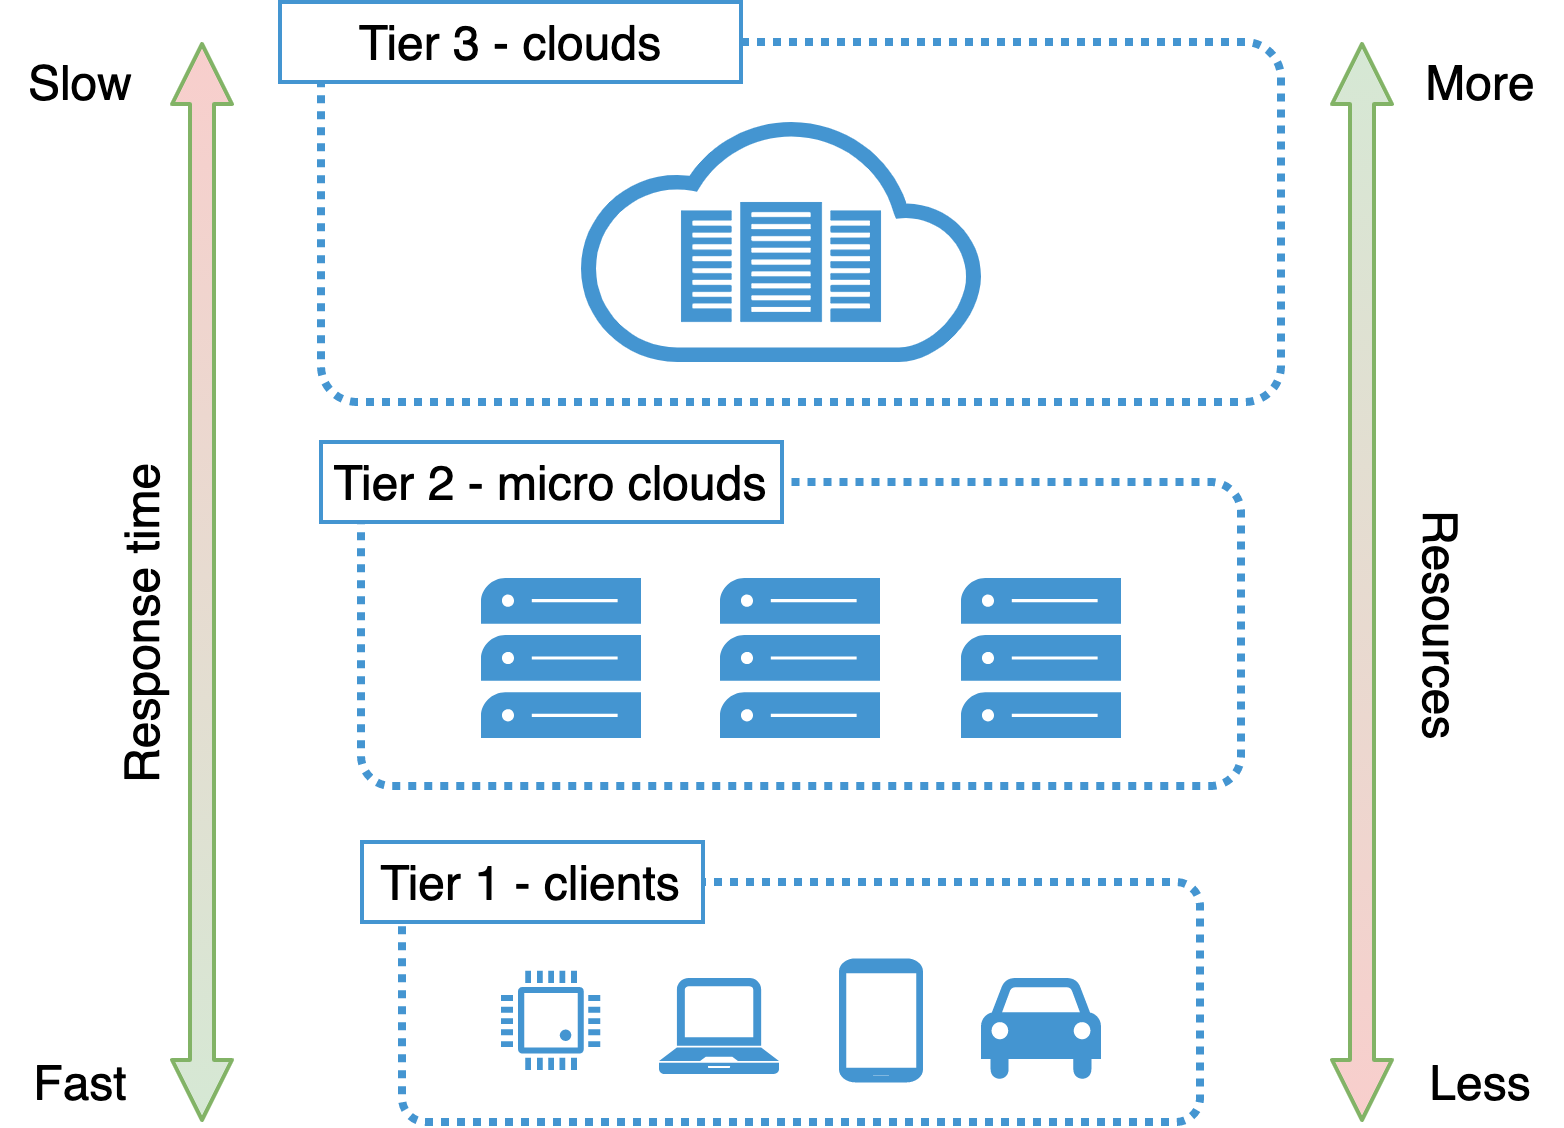
\includegraphics{images/Figure9}
	\end{center}
	\vspace{-0.5cm}
	\caption{Three tier architecture, with the response time and resource availability}
	\label{fig:fig9}
\end{figure}

\noindent
On lower levels, response time is the fastest, since data is processed closer to the source. At the same time, there is a limited storage capacity and processing power. As we go on the upper tiers, there is more and more storage capacity and processing power, but the response time is higher and higher, especially when distance and huge volumes of data that need to be moved to the cloud are considered.

In everything as a service model~\cite{DuanFZSNH15}, ECC as a service fits in between CaaS and PaaS, depending on the user needs. 
%
%
\section{Separation of concers}\label{sec:separation_of_concerns}
%
In his work, Jin et al.~\cite{JinCJL14} introduces three core concepts to fully describe physical services, and specifies their relationships. Concepts that authors propose are: \textbf{(1)} Devices, \textbf{(2)} Resources, and \textbf{(3)} Services. This separation is interesting because we can rely on it in a geo-distributed environment, to describe SoC for $\upmu$Cs.

One of the most important part of every system, is the SoC model. This is especially important if a platform to be offered as a service is going to be created. With some adaptations, our SoC model can be based on concepts proposed by Jin et al.~\cite{JinCJL14} in three layers, as depicted in Figure~\ref{fig:fig10}. 

The layer on the very bottom of the three-tier architecture (see~Figure~\ref{fig:fig10}) consists of various devices. These devices are important because they represent main \textit{data creators} but at the same time, they are main \textit{services consumers}. 

The layer in the middle (see~Figure~\ref{fig:fig10}) represents resources or EC nodes. These resources have a very important spatial feature, and as such, they indicate the range of their hosting devices~\cite{JinCJL14}. This means that the developers at any given time must know the topology of the system, the resource spread, and utilization across clusters. Besides that main information, users must know the state and health of every application\label{soc:resources}. If some EC node desires to be a part of the system, a node must obey four simple rules:

\begin{enumerate}[start=1,label={(\bfseries \arabic*)}]
\item A node must run an operating system with a usable file system;
\item A node must be able to run some isolation engine for applications, for example, containers or unikernels;
\item A node must have available resources for utilization so that applications can be run or data stored;
\item A node must have internet connection.
\end{enumerate}

\noindent
One thing that is important to notice, is that all nodes in clusters, regions, and topologies are \textbf{equal} and there are \textbf{no special nodes}. Every node that joins the system must be able to store and process information.

Last but certainly not least layer represents services. These services expose resources through some interface and make them available over the internet~\cite{JinCJL14}. These services respond to the client requests immediately, if possible, or cache information~\cite{SatyanarayananBCD09,YaoXWYZP20} for future use. Unlike the previous two layers, services have one specific feature and span over two tiers of the system (see~Figure~\ref{fig:fig10}):

\begin{enumerate}[start=1,label={(\bfseries \roman*)}]\label{services}
	\item Services that exist in the $\upmu$C, and they are responsible for filtering and data pre-processing before sending it to the cloud. Or cache information that was not available on a previous user request for some future use;
	\item Services in the standard cloud that should be able to accept pre-processed data, and they are responsible for computation and storage that is beyond the capabilities of ECC nodes. Services in the cloud should be able to take direct requests from the clients in a case when something catastrophic happens to the $\upmu$C that is close to the user, and it is not able anymore to accept user requests.
\end{enumerate}

\noindent
This kind of services separation creates new application model that we present in detal in the secion~\ref{sec:application_model}. 

Figure~\ref{fig:fig10}. shows the proposed SoC for every layer of the ECC as a service model.

\begin{figure}[H]
	\includegraphics[width=\linewidth]{images/FIG1}
	\vspace{-0.7cm}
	\caption{ECC as a service architecture with separation of concerns.}
	\label{fig:fig10}
\end{figure}
%
%
\section{Applications Model}\label{sec:application_model}
%
Modern-day applications that should run in the cloud are advised to follow the cloud-native model~\cite{GannonBS17}. With this approach, we get applications that are easier to scale, more available, and less error-prone when compared to traditional web applications~\cite{GannonBS17}. 

Satyanarayanan et al. present the edge-native applications model~\cite{SatyanarayananK19} that should use the full potential of EC infrastructure, and keep good features of their cloud counterparts. 

When we introduced SoC for the $\upmu$C model (see page~\pageref{services}), we described services that have one specific feature, and that is that these services span over two tiers of the system. This information is crucial for application development because we want to use the full potential of formed infrastructure, and keep good features of their cloud counterparts.

To satisfy the previously defined SoC model (see page~\pageref{services}), existing applications can be split into the \textbf{front} and \textbf{back} processing services. The front processing service is an edge-native application running inside some previously formed cluster to minimize latency, while the back service runs in the traditional cloud as a cloud-native application to leverage greater resources.

The front processing service will handle user requests coming to the nearby cluster, and communicate with the back processing services when needed to synchronize the pieces of information, cache data, or pass filtered or pre-processed data. Separation like that gives developers better flexibility and large design space when creating and optimizing their workloads. At the same time, it ties together the traditional clouds and edge comuting into one coherent system. Figure~\ref{fig:fig29} shows $\upmu$C applications model that tides edge and traditional cloud applicatoins.

\begin{figure}[H]
	\begin{center}
		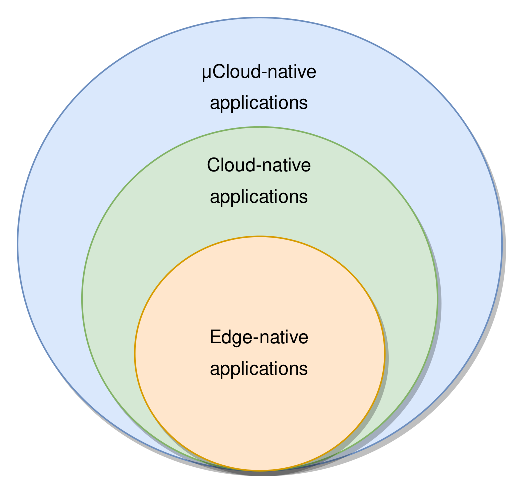
\includegraphics[scale=0.85]{images/Figure29}
	\end{center}
	\vspace{-0.7cm}
	\caption{$\upmu$C applications model tides traditional clouds and edge computing applications}
	\label{fig:fig29}
\end{figure}

With this model, we venture even deeper into understanding and applying the concept of \textbf{data locality} (see page~\pageref{ds:data_locality}). Since we have front and back processing services, we are committed to doing processing data closer to their source, instead of moving data to the cloud. This reduces latency and saves some users money on storing and processing unnecessary data.
%
%
\subsection{Execution models}\label{sec:execution_models}
%
Frontend services model should be packed in some standard way~\ref{sec:virtualization_techniques} and deployed in the wild, as an event-driven application, with the subscription policy to message streams, or infinite sequences~\cite{Rutten03} using topics~\cite{inproceedingsBeck}. The processing strategy is in the developer's hands, depending on the nature of the use-case. 

If a service is subscribed to some stream using a topic, for example, it is natural that events appear in their stream. There are two strategies for building a large-scale time-ordered event system:

\begin{enumerate}[start=1,label={(\bfseries \arabic*)}]
	\item \textbf{Fan out on write}, with this strategy, every service has some form of inbox, and when an event appears for some topic, that data is copied to every service that is subscribed to that topic. With these options, reads are fast, but writes are not. The more subscribers to the topic, the longer it takes to persist all updates; 
	\item \textbf{Fan in on read}, with this strategy, every topic has a sort of outbox where it can store data. When services read their streams, the system will read the recent data from the outboxes. Writes are fast, and used storage is minimal, but reads are difficult because to do this properly on a request-response deadline is not a trivial task to do.
\end{enumerate}

\noindent 
To implement those ideas without complicated synchronization, CRDTs could be used~\ref{crdts}. Companies like Soundcloud and Bet365 are already using them for the same or similar tasks.

Some examples of applications may include:

\begin{enumerate}[start=1,label={(\bfseries \arabic*)}]
	\item \textbf{Events} that notify users if some value is above or below some defined threshold; 
	\item \textbf{Stream} or processing data as it comes to the system;
	\item \textbf{Micro-batch} processing delivers data more slowly than real-time data processing but faster than typical batch processing. It is performed in smaller batches, than traditional batch processing. This type of processing is for applications that require high-throughput processing over large data streams~\cite{AbdelhamidMDA20};
	\item \textbf{Batch} does processing in predefined times over some bigger collection of data;
	\item \textbf{daemons} or processing that are that do some tasks or executions in the background without explicit user intervention, usually their execution could be time defined but it is not mandatory;
	\item \textbf{Services} or applications that would operate over standard request-response model or some variation of that protocol. For example, the NATS messaging system has a request-reply form implemented over topics;
	\item \textbf{Other}, something that falls outside these models, or it is a composition of multiple operations at once. This can be represented as a function composition in mathematics:
	
	\begin{equation}~\label{size:eq3}
		(f \circ g)(x) = f(g(x))
	\end{equation}
	\myequations{Function composition.}
	
	This type should get events from some topic as they arrive, and a user can define his strategy what needs to be done and how it needs to be processed. Users can contact other existing services or combine them (eq.~\ref{size:eq3}), and the user is responsible for optimization;
\end{enumerate}

\noindent
These types of applications could be implemented in many ways like those discussed in section~\ref{sec:microservices}, or some adapted variant of those models, and should have a clear communication interface offered to users or applications and other services. 

Users should be given the option to develop their applications in various available languages, not forcing them to use a strict one. Users must also be advised about outcomes of their choice. 

For example, some languages might be slower or use more resources than others due to virtual machine execution, or some other tooling that is required to be started as well. The second important thing would be that users can do proper logging and tracing of their services. If something fails, the user must be able to go over the logs and traces to find problems.
%
\subsection{Packaging options}\label{sec:packaging}
%
Because of their nature, $\upmu$Cs could be most likely composed of ARM devices. These devices in many cases are not able to run full VMs because of their hardware restrictions. In recent years there have been advances in VMs technology and its ability to run VMs on ARM devices. In~\cite{Ding12armvisor} Ding et al. show such possibility to run VMs on ARM devices.

But even if VMs are fully compatible with ARM devices, we still inherit VMs large footprint, already discussed in section~\ref{sec:virtualization_techniques} if we try to use them $as is$.

On the contrary, containers, and unikernels give us \textbf{more or less} the same functionality, but use fewer resources, which means that more services can be run in containers and even more in unikernels. Until unikernels are fully ready to be used, though, they will fall in nice to have a category, and we should stick to containers. But even with containers we need to be aware of their limitations and pitfalls and know that there is no comprehensive solution and there is not just one solution for all scenarios.

At the moment, containers are a more mature solution than unikernels and require fewer resources than VMs. On top of that, there are numerous tools already existing using containers that could be utilized. Knowing all this, at the first stages of $\upmu$Cs, containers should be an option to go. 

In~\cite{inproceedingsSimic3} Simi\' c et al. show benefits of using containers in large scale edge computing systems from the theoretical point of view, by looking into architecture difference. Authors focus on differences between VMs and containers in cases where services need to run on ARM devices with limited resources.

In terms of boot times, throughput, and memory consumption, unikernels are famous for providing excellent performance~\cite{abs-2104-12721}. In the future and when unikernels are more matured and tested, they could be used for particular use-cases and applications, especially like events or serverless implementations. The containers will probably not be fully replaced, but they can co-exist with unikernels in some cases where more control over running a single function is needed.

Like any other system, users can create variants of the systems and different flavors optimized for certain solutions. In that cases, they may favor one solution over the other one. In general, containers and unikernels should be the preferred way to package, run, and distribute user applications in a $\upmu$Cs environment.
%
%
\section{As a service model}\label{sec:as_a_service_model}
%
Users should be able to develop their applications using familiar models, depending on their needs. Depending on how much control a user requires over the process of service scheduling, resource selection, etc. three models can be distinguished:
 
\begin{enumerate}[start=1,label={(\bfseries \arabic*)}]
	\item \textbf{Micro PaaS or $\upmu$PaaS}, where the platform does all the management and offers a simple interface for developers to deploy their applications. This model is similar to PaaS, and the only difference is that this runs in $\upmu$C and should synchronize with CC;
	\item \textbf{Micro CaaS or $\upmu$CaaS}, if users require more control over resource requirements, deployment, and orchestration decisions. This model is similar to CaaS (or even IaaS), and the only difference is that this runs in $\upmu$C and should synchronize with CC;
	\item \textbf{Micro SaaS or $\upmu$SaaS}, with this option, data is not synchronized with the CC, but all processing and storage is done in the $\upmu$C. As such, this option should be used vigilantly.
\end{enumerate}

\noindent
It is important to note, that both variants, \textbf{mCaaS} and \textbf{mPaaS}, should \textbf{not} stand alone, at least not for now. Using \textbf{mSaaS} is not being advised for now, since that would require that the whole application be running \textbf{only} in the $\upmu$Cs. In the future, when EC nodes gain more power and storage, this might change. \textbf{mSaaS} as an option should more investigated in the future.

Both options, \textbf{mCaaS} and \textbf{mPaaS}, could be included, and a part of any cloud model (se Section~\ref{sec:cloud_computing}), multi-cloud or offered separately.
%
%
\section{Immutable infrastructure}\label{sec:immutable_infrastructure}
%
This thesis proposes a DS model that is built with a three-tier architecture that should operate in the geo-distributed environment. 

We believe that \textbf{immutable deployment} model would be a good fit for such environnment. It will simplify the deployment process, since we want to rely on \emph{atomic operations} and do not want to leave the misconfigured system at any level~\cite{SimicSensors}. If something like that happens, there will be a problem that would be hard to properly track, address and resolve.

Geo-distributed $\upmu$Cs model that is described in this chapter should operate in two levels of deployment that are built one on top of the other:

\begin{enumerate}[start=1,label={(\bfseries \arabic*)}]
	\item \textbf{Infrastructure deployement}, update and change should be atomic and immutable. Users should do changes declaratively -- mutations of the system, by telling the system what the new state should be, and let the system figure out the best way how to do user-specified changes. In this category, we can account for any change that is doing on the cluster, region, or topology that user(s) operate on. For example create the new cluster, region, topology, or doing configurations of the setup system. The only change that could be done by imperative strategy updates on the nodes themselves. But even for this strategy, it would be beneficial if we could use declarative way \textbf{if possible}. It is important to notice that \textbf{mutation} does not mean in place change, but just the name of the operation. This deployment strategy is reserved for operations people or (eg. DevOps or SREs), but if the company or team is small any developer could do this. Developers should not be dealing with this part of the deployment;
	\item \textbf{Services deployment}, makes sense only if the previous action is taken. We must have infrastructure already set up, to put any sort of services (applications) into the system. Like the previous model, this should be done declaratively as well, and all changes should be done immutably without an in-place change. The user should specify his new state or \say{view of the word} declaratively and let the system do all the changes he wants. All user services should be packed as described in section~\ref{sec:packaging} because this simplifies the way services are put to the nodes. When done properly, this allows operations people to do faster changes with almost zero downtime deployments with all strategies already discussed in section~\ref{sec:deployment}. This part of the deployment should be done by developers since they did implementation and testing. They know how many resources they need for their service, what type of service they had developed. This deployment could be done in collaboration between operations and developers if a company is big or time is properly separated.
\end{enumerate}

\noindent
It is important to notice, that both deployments should be closely followed, for possible errors and problems so that users can act accordingly. These deployment messages, logs, and traces~\cite{36356} should be stored in a centralized log system, for convenient lookup, alerting, and reporting.

Separation like this simplifies deployment and usage for both application development spectrums: 

\begin{enumerate}[start=1,label={(\bfseries \roman*)}]
	\item \textbf{Operations} who should be dealing with infrastructure deployment, tooling set up, applications deployment, monitoring, and in the general health of applications and infrastructure;
	\item \textbf{Developers} who should be dealing with the development of the services, their interactions, and cloud to $\upmu$C and vice-versa synchronization.
\end{enumerate}

\noindent
Only with tight collaboration with those two development roles, such a complex system like one presented in this chapter can be alive, well, and serving user requests without collapse.

It is important to note that every action in the system should be logged and traced properly. Since we are dealing with multi-tier architecture, a chance that something will fail is increased. Logs and traces should be available to operations people who are responsible for the infrastructure maintenance. 

At the same time, actions should be traced by the company that offers these $\upmu$Cs. For security reason, any of these logs and traces should not be visible to others \textbf{but} responsible individuals, and the level of details and personal pieces of information should be different.
%
%
\subsection{Deployment in micro clouds}~\label{sec:dep_mc}
%
As described in section~\ref{sec:deployment}, there are a few options when it comes to setup and deployment of infrastructure and/or applications. Let us explore interesting options how both \textbf{(1)} infrastructure, and \textbf{(2)} services could be deployd in $\upmu$Cs.

\emph{Rolling update} strategy minimize the downtime, at the cost of update speed. 

Figure~\ref{fig:fig24} shows flow chart for \emph{rolling update} in $\upmu$Cs for both services and infrastructure.

\begin{figure}[H]
	\begin{center}
		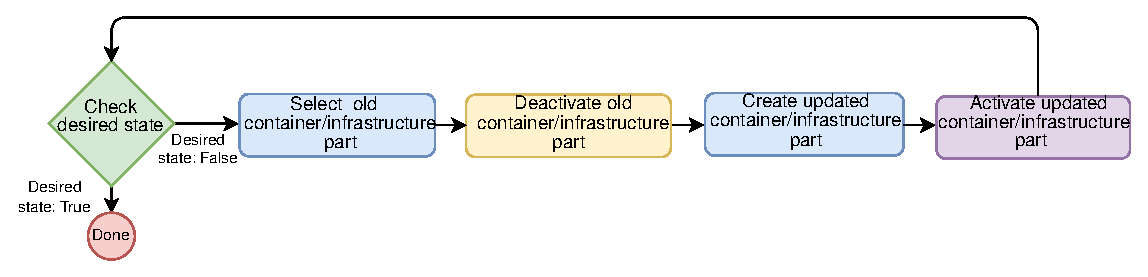
\includegraphics[width=\columnwidth]{images/Figure24}
	\end{center}
	\vspace{-0.5cm}
	\caption{Rolling update flow chart}
	\label{fig:fig24}
\end{figure}

\noindent
On the other side of the spectrum, the users should be able to choose the \emph{recreation} strategy as well. This strategy will causes higher downtime, but it will do updates quickly.~\label{sec:recreation} 

Figure~\ref{fig:fig27} shows flow chart for \emph{recreation strategy} in $\upmu$Cs for both services and infrastructure.

\begin{figure}[H]
	\begin{center}
		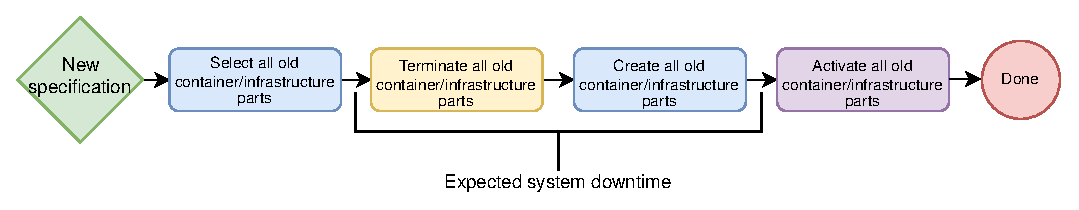
\includegraphics[width=\columnwidth]{images/Figure27}
	\end{center}
	\vspace{-0.5cm}
	\caption{Recreation strategy update flow chart}
	\label{fig:fig27}
\end{figure}

\noindent
The third strategy is the \emph{canary update} strategy. This strategy offers a partial update process allowing to test new environment version , without a commitment to a full rollout. 

This strategy comes handy when we want to test how your services perform in real-life scenarios with production data and users, allowing the revert to previous version fast.

In this strategy, the deployment creates a few new artifacts while keeping most artifacts on the previous version. The ration between new and previous version should be provided by the user. After the test, we can go either direction: \textbf{(1)} full rollout, \textbf{(2)} revert to previous version. Both directions are predicated by the results of the test.

Figure~\ref{fig:fig28} shows chart for the \emph{canary update} strategy deployment.

\begin{figure}[H]
	\begin{center}
		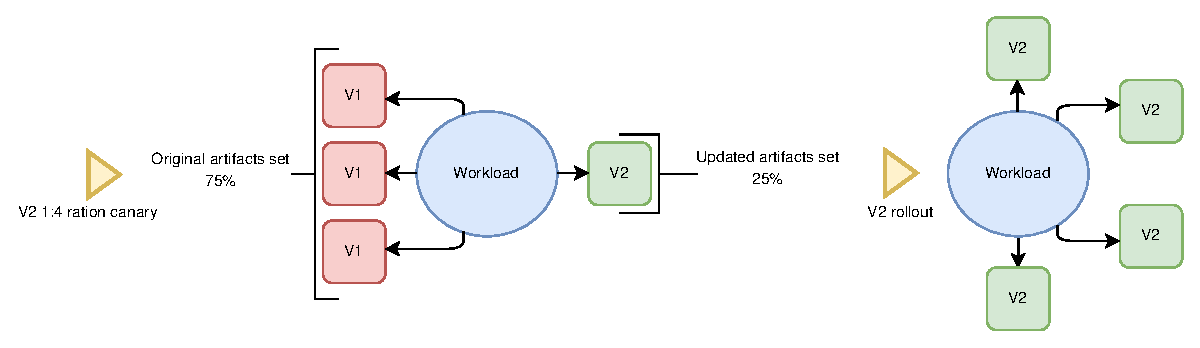
\includegraphics[width=\columnwidth]{images/Figure28}
	\end{center}
	\vspace{-0.5cm}
	\caption{Canary update 1:4 ration update chart}
	\label{fig:fig28}
\end{figure}

%
%
\section{Formal model}\label{sec:formal_model}
%
Ensuring the reliability and correctness of any DS is a very difficult task, and should be mathematically based. Formal methods are techniques that allow us to create specifications and verification of complex (software and hardware) systems based on mathematics and formal logic. There are several options for how to formally describe DS: TLA+~\cite{YuML99}, $pi$ calculus~\cite{0018113}, combinational topology~\cite{Upadhyay16}, asynchronous session types (MST)~\cite{HondaYC08}, etc. 

Unfortunately, because of their nature DS cannot always be formally described by any of the existing techniques. There are a lot of variables that could influence this. But if the nature of the DS that is developing is such that can be formally described, it is recommended and beneficial. A formally described and correct model can save hours, days, and even months of hard debugging, testing to reveal all bugs and problems in the system that may only happen in some specific circumstances that are hard to initiate.

Infrastructure deployment will not happen overnight, and it might take years. It might not be started at all until the whole process is trivial \cite{SatyanarayananBCD09}, and this is a complicated task~\cite{JararwehDAAAB16}. Because of those properties, the key problem that needs to be resolved is how to simplify ECC or $\upmu$C management. The naive approach would require going to every node and do it manually. This process is super tedious and time-consuming, especially if we consider a geo-distributed environment. 

In such a complex environment, formal models are of great help if we can model and prove that protocols that the system relies on are correct. The system we propose tackles this issue using remote configuration and it relies on four formally modeled protocols:

\begin{enumerate}[start=1,label={(\bfseries \arabic*)}]
	\item \textbf{Health-check protocol} informs the system about state of every node (see Section~\ref{sec:health_check_protocol});
	\item \textbf{Cluster formation protocol} forms new clusters dinamicaly (see Section~\ref{sec:cluster_formation_protocol});
	\item \textbf{Idempotency check protocol} prevents system from creating existing infrastructure (see Section~\ref{sec:idempotency_protocol});
	\item \textbf{List detail protocol} shows the current state of the system to the user (see Section~\ref{sec:list_detail_protocol});
\end{enumerate}

\noindent
These three protocols are based on the geo-distributed Infrastructure deployment.
%
%
\subsection{Multiparty asynchronous session types}\label{sec:multiparty}
%
Communication protocols that operate from node to the system can be modeled using~\cite{HuY17}, an extension of \emph{MPST}~\cite{HondaYC08} -- a class of behavioral types specifically designed for describing distributed protocols that rely on asynchronous communications. 

The type specifications give us one additional benefit. They are not only useful to formally describe protocols, but also reliable for a modeling-based approach developed in~\cite{HuY17} to validate our protocols are they satisfy multiparty session types safety (there is no reachable error state) and progress (an action is eventually executed, assuming fairness).

The modeling process is done in two steps.

\begin{enumerate}[start=1,label={(\bfseries \arabic*)}]
	\item \textbf{The first step} in modeling the communications of a system using MPST theory is to provide a \emph{global type}, that is a high-level description of the overall protocol from the neutral point of view. Following~\cite{HuY17}, the syntax of global types are constructed by:
	
	\begin{equation}
	\G \; ::= \;
	\{\pp\dagger\pq_i{:}\ell_i(\T_i).\G_i\}_{i\in I}  \quad | \quad 
	\mu \ty.\G \quad | \quad 
	\ty \quad | \quad
	\tend
	\end{equation}
	\myequations{Global type construction}
	
	\noindent
	where $\dagger\in\{\to, \twoheadrightarrow\}$ and $I\not=\emptyset$. 
	In the above, $\{\pp\dagger\pq_i{:}\ell_i(\T_i).\G_i\}_{i\in I}$
	denotes that \emph{participant} $\pp$ can send (resp. connects) to one of the participants $\pq_i$, 
	for $\dagger=\to$ (resp. $\dagger=\twoheadrightarrow$), 
	a \emph{message} $\ell_i$ with the \emph{payload} of \emph{sort} $\T_i$, 
	and then the protocol continues as prescribed with $\G_i$.  
	$\mu \ty.\G_1$ is a recursive type, and $\ty$ is a recursive variable, 
	while $\tend$ denotes a terminated protocol. We assume all participants are (implicitly) disconnected at the end of each session (cf.~\cite{HuY17}).
	
	The advance of using approach of~\cite{HuY17}, when compared to standard MPST (e.g.,~\cite{HondaYC08}),
	is in a relaxed form of choice (a participant can choose between sending to different participants), 
	and, $\twoheadrightarrow$, that explicitly connects two participants, hence (possibly) dynamically 
	introducing participants in the session.
	Both of these features will be significant for modeling our protocols (we will return to this point);
	
	\item \textbf{The second step} in modeling protocols by MPST is providing a syntactic projection of the protocol onto each participant as a local type, that is then used to
	type check the endpoint implementations.  
	We use the definition of projection operator given in~\cite[Figure \ref{fig:fig2}]{HuY17}. 
	In essence, the projection of global type $\G$ onto participant $\pp$ can result in 
	$\ST_\pp=\pq{!}\ell(\T)\ldots$ (resp. $\ST_\pp=\pq{!!}\ell(\T)\ldots$) 
	when $\G=\pp\to\pq{:}\ell(\T)\ldots$ (resp. $\G=\pp\twoheadrightarrow\pq{:}\ell(\T)\ldots$), 
	and, dually, $\ST_\pp=\pq{?}\ell(\T)\ldots$ (resp. $\ST_\pp=\pq{??}\ell(\T)\ldots$) when $\G=\pq\to\pp{:}\ell(\T)\ldots$ 
	(resp. $\G=\pq\twoheadrightarrow\pp{:}\ell(\T)\ldots$), 
	while the projection operator ``skips'' the prefix of a global type if participant $\pp$ is not mentioned neither as sender nor as receiver. Furthermore, a local type must be represented by the following syntax:
	
	\begin{equation}
	\ST \; ::= \; 
	{+}\{\pq_i\alpha\ell_i(\T_i).\ST_i\}_{i\in I}  \quad | \quad 
	\mu \ty.\ST \quad | \quad 
	\ty \quad | \quad
	\tend
	\end{equation}
	\myequations{Local type representation syntax.}
	
	\noindent
	where $\alpha\in\{{!}, {!!}\}$ or  $\alpha\in\{{?}, {??}\}$ (in which case $\pq_i=\pq_j$ must hold for all $i,j \in I$, to ensure consistent external choice subjects, cf.~\cite[Page 6.]{HuY17}), and $I\not=\emptyset$.
	Interested reader can find details in~\cite{HuY17}.
\end{enumerate}

\noindent
For simplicity reasons, we will consider that all participants are communicating in a single private session. All sent messages, but not yet received, are buffered in a single queue that preserves their order. The order is preserved only for pairs of messages having the same sender and receiver, while other pairs of messages can be swapped since these are asynchronously independent.
%
%
\subsection{Health-check protocol}\label{sec:health_check_protocol}
%
Nodes that exist in the clustered environment usually have a channel where they can send metrics and other data in a form of a health-check mechanism. This channel could be used this channel to reach nodes to send some actions to them, for example, a cluster formation message. 

In figure~\ref{fig:fig6}. a low-level health-check protocol between a single node and the rest of the system can be seen. This process involves the following participants: Node, Nodes, State, and Log.

\begin{figure}[H]
	\begin{center}
		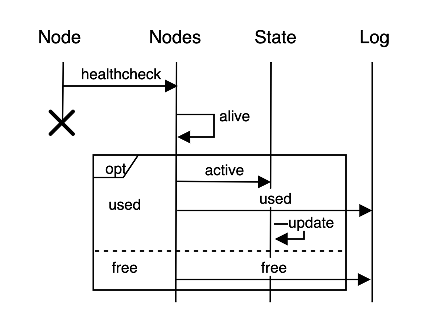
\includegraphics[scale=0.75]{images/FIG2}
	\end{center}
	\vspace{-0.7cm}
	\caption{Low level health-check protocol diagram.}
	\label{fig:fig6}
\end{figure} 

\noindent
These participants included in Figure~\ref{fig:fig6} follow the health-check protocol~\label{informal_description_health-check} that is informally described below:

\begin{enumerate}[start=1,label={(\bfseries \arabic*)}]
	\item \textbf{Node} sends a health-check signal to the Nodes service;
	\item \textbf{Nodes} accept health-check signals from every node, update node metrics and if node is used in some cluster, inform that cluster about the node state;
	\item \textbf{State} contains information about nodes in the clusters, regions and topologies;
	\item \textbf{Log} contains records of operations. Users can query this service. 
\end{enumerate}

\noindent
Nodes service will be informed about node existence on his health-check ping. However, the system state will not be updated, changed, or even informed about this ping if the node is not used in some cluster.

In the following algorithm~\ref{alg:alg1} steps required by the system to determine if the node is free or used, and how node information is stored, are described.

\begin{algorithm}[H]
	\SetAlgoLined
	\SetKwInOut{Input}{input}
	\Input{event, config}
	\uIf{isNodeFree(event.id)}{
		\eIf{exists(event.id)}{
			renewLease(event.id, config.leaseTime)\;
			updateData(event.id, event.data)\;
		}{
			leaseNewNode(event.id, config.leaseTime, event.data)\;
			saveMetrics(event.id, event.metrics)\;
		}
	}\uElseIf{isNodeReserved(event.id)}{
		updateData(event.id, event.data)\;
	}\Else{
		renewLease(event.id, config.leaseTime)\;
		updateData(event.id, event.data)\;
		saveMetrics(event.id, event.metrics)\;
		sendNodeACK(event.id)\;
	}
	\caption{Health-check data received}
	\label{alg:alg1}
\end{algorithm}

\noindent
To formally describe servers or nodes (terms are used interchangeably) properties in the system, set theory could be used. At the beginning, the system will have an empty server set $S$ denoted with $S=\emptyset$. To determine node state, we could use existing node properties. One approach may be that we use a node-id structure, for example. 

Whatever approach is used, free nodes can be formally described as follows:

\begin{definition}
	Nodes are free if and only if (henceforth iff) they do not belong to any cluster.
\end{definition}

\noindent 
If \textbf{node-id} is taken, for example, when the new health-check message from the particular node is received, \textbf{node-id} structure will determine the node state. When the node is free, it will home some random or user-defined id, while when it is used in some cluster, the node-id structure will reflect this.\\

If, for example, there are $n$ free nodes in the wild, this can be denoted with $s_i$, where $i\in\{1, \ldots, n\},$. If all of them send the health-check ping to the system, we need to determine their state. If a node $s_i$ is free, we should add it to the server set, and thus we have:

\begin{equation}
	S_{\mathit{new}} = S_{\mathit{old}} \cup \bigcup%\limits
	_{i=1}^{n} \{s_i\}
\end{equation}
\myequations{Extending free servers set.}
 
\noindent 
It is important to notice, that the order in which messages arrive is not important. The only thing that is important is that every message eventually comes into the system. Node roles in the system can now formally be defined like:

\begin{definition}
	All nodes in the system are equal, no matter if they are a part of some cluster or if they are not.
\end{definition}

\noindent
The previous definition gives us a strong background in the further formal definition of the system because the only thing that should be cared about is that node is alive and well, and that it is ready to accept some jobs.\\

We described in algorithm~\ref{alg:alg1} how the system stores the node data, but also how to determine if the node is free or used using the node-id structure. Every node $s_i$ in the system that is part of the server set $S$ could be described as a tuple $s_i = (L, R, A, I)$, where:

\begin{itemize}
	%
	%
	\item $L$ is a set of ordered key-value pairs: $L = \{(k_1,v_1),\ldots ,(k_m,v_m)\}$ where $k_i \not= k_j$, for each $i,j\in \{1, \ldots , m\}$ such that $i\not= j$. $L$ represents node labels or server-specific features.  
	Labels were based on Kubernetes~\cite{RossiCPN20} labels concept, which is used as an elegant binding mechanism for its components.
	%
	%
	\item $R$ is a set of tuples $R = \{(f_1,u_1,t_1),\ldots ,(f_m,u_m,t_m)\}$ representing node resources, where $f_i,u_i,t_i$, for $i\in\{1,\ldots,m\}$ are as follows:
	\begin{itemize}
		\item $f_i$ is the free resource value, 
		\item $u_i$ is the used resource value, and 
		\item $t_i$ is the total resource value. 
	\end{itemize}
	%
	%
	\item $A$ is a set of tuples $A = \{(l_1,r_1,c_1,i_1), \ldots ,(l_m,r_m,c_m,i_m)\}$, representing running applications, where $l_j,r_j,c_j,i_j$, for $j\in\{1,\ldots,m\}$, are as follows: 
	\begin{itemize}
		\item  $l_j$ represents labels, the same way we used for node labels, 
		\item $r_j$ is the resource set application requires, 
		\item $c_j$ is the configuration set application requires, and 
		\item $i_j$ is the general information like name, port, developer. 
	\end{itemize}
	%
	%
	\item $I$ represents a set of general node information like: name, location, IP address, id, cluster id, region id, topology id, etc.
\end{itemize}

\noindent
If we want to assign $m$ (fresh) labels to the $i_\mathit{th}$ server, we start with empty labels set $s_i[L]=\emptyset$, then we add labels to server. Therefore, we have 

\begin{equation}
	s_i[L]_\mathit{new} = s_i[L]_\mathit{old} \cup \bigcup%\limits
	_{j=1}^{m} \{(k_j,v_j)\
\end{equation}
\myequations{Extending label set.}

\noindent
We can now formally define the number of labels per single server $s_i$ in the system like:

\begin{definition}
	Every node from the server set $S$ \textbf{must have} \emph{non-empty} set of labels. The number of labels for every server $s_i$ in the server set $S$ may vary.
\end{definition}

\noindent
Since labels are an important part of the system (more in future sections), they should be picked carefully and agreed on upfront. It should also be possible to change them if such a thing is required. 

Labels should stick out some distinctive features of the node, that might be valuable for developers or administrators to target. For example, server resources, server features (e.g., SSD drive), geolocation, etc. They can be created as follows:

\begin{definition}
	Labels are created using arbitrary long alphanumeric text, for both keys and values, separated by colon sign. For example os:linux, arch:arm, model:rpi, cpu:$2$, memory:$16$GB, disk:$300$GB.
\end{definition}

\noindent
Following all things presented above, we can now give a formal description for the low-level health-check communication protocol (see Figure~\ref{fig:fig6}). The global protocol $\G_1$ (given bellow) conforms the informal description given at page~\pageref{informal_description_health-check}: $\mathtt{node}$ connects $\mathtt{nodes}$ with $\mathit{health{\_}check}$ message and a payload of type $\T_1$ required by the system to properly register node into the system. 

Based on the received information, $\mathtt{nodes}$ {\bf either} connect $\mathtt{state}$ with $\mathit{active}$ message, informing the node status alongside payload typed with $\T_2$ (containing informations required by the system to properly register active health-check sender), and then also connect $\mathtt{log}$ with the same message, {\bf or} directly connect $\mathtt{log}$ informing the node is $\mathit{free}$.
\begin{align*}
\G_1 = & 
\mathtt{node} \twoheadrightarrow \mathtt{nodes}{:}\mathit{health{\_}check}(\T_1).\\
& \hspace{2mm}
\left\{
\begin{array}{@{}l@{}}
\mathtt{nodes} \twoheadrightarrow \mathtt{state}{:}\mathit{active}(\T_2).\mathtt{nodes}\twoheadrightarrow \mathtt{log}{:}\mathit{used}(\T_2).\tend\\
\mathtt{nodes}\twoheadrightarrow \mathtt{log}{:}\mathit{free}(\T_2).\tend
\end{array} \right.
\end{align*}
\myequations{Health-check global protocol.}

Notice that in $\G_1$ we indeed have a choice of $\mathtt{nodes}$ sending either to $\mathtt{state}$ or to $\mathtt{log}$. Such communication patterns are impossible to be modeled using just standard MPST approaches. 
Also, notice that $\mathtt{state}$ will be introduced into the session only when receiving from $\mathtt{nodes}$. 
Hence, if the session after the first ping from $\mathtt{node}$ to $\mathtt{nodes}$ proceeds with the second branch (i.e., connecting $\mathtt{nodes}$ with $\mathtt{log}$) then $\mathtt{state}$ is not considered as stuck, as it would be in standard MPST, such as, e.g.,~\cite{HondaYC08}, but rather idle. 

Projecting global type $\G_1$ onto participants $\mathtt{node}, \mathtt{nodes}, \mathtt{state}$ and $\mathtt{log}$ we can then get local types as follows:
\begin{align*}
\ST_\mathtt{node}  & = 
\mathtt{nodes}{!!}\mathit{health{\_}check}(\T_1).\tend
\end{align*}
\begin{align*}
\ST_\mathtt{nodes} & = 
\mathtt{node}{??}\mathit{health{\_}check}(\T_1). \\
& \hspace{-2mm}
{+} 
\left\{
\begin{array}{@{}l@{}}
\mathtt{state}{!!}\mathit{active}(\T_2).\mathtt{log}{!!}\mathit{used}(\T_2).\tend\\
\mathtt{log}{!!}\mathit{free}(\T_2).\tend
\end{array} \right.
\end{align*}
\begin{align*}
\ST_\mathtt{state} &= 
\mathtt{nodes}{??}\mathit{active}(\T_2).\tend
\end{align*}
\begin{align*}
\ST_\mathtt{log} &= 
{+}
\left\{
\begin{array}{@{}l@{}}
\mathtt{nodes}{??}\mathit{used}(\T_2).\tend\\
\mathtt{nodes}{??}\mathit{free}(\T_2).\tend
\end{array} \right.
\end{align*}
\myequations{Health-check global protocol projection.}
\noindent
where, for instance, type $\ST_\mathtt{nodes}$ specifies $\mathtt{nodes}$ can receive the ping message from $\mathtt{node}$, after which it will dynamically introduce either $\mathtt{state}$ or $\mathtt{log}$ into the session, where in the former case it also connects $\mathtt{log}$ (but now with message $\mathit{free}$). 
%
%
\subsection{Cluster formation protocol}\label{sec:cluster_formation_protocol}
%
Another communication protocol that the system relies on, appears in the cluster formation process, where users can form new clusters dynamically. Two different actions are distinguished:

\begin{enumerate}[start=1,label={(\bfseries \arabic*)}]
	\item The first action is user-system communication. Here user sends query parameters to the system to obtain a list of available nodes that satisfy specified query parameters;
	\item The second action is a little bit more complicated than the previous one, and it starts when the user sends a message to the system with a new assembly specification. In this setting, the system involves participants: User, Queue, Scheduler, State, Nodes, Log, and NodesPool. These participants need to cooperate to successfully form new clusters, regions, or topologies dynamically, adhering to the scenario shown in Figure \ref{fig:fig7}.
\end{enumerate} 

\begin{figure}[H]
	\begin{center}
		\includegraphics[scale=0.7]{images/FIG3}
	\end{center}
	\vspace{-0.7cm}
	\caption{Low level cluster formation communication protocol diagram.}
	\label{fig:fig7}
\end{figure}

\noindent
These participants included in Figure~\ref{fig:fig7} follow the cluster formation protocol that is informally described below:

\begin{enumerate}[start=1,label={(\bfseries \arabic*)}]
	\item \label{cluster_formation_informal_description} \textbf{User} query Nodes service, based on some predefined query parameters. User sends a new creation message to Queue. User either gets response \textit{ok} if the message is accepted or \textit{error} if the message cannot be accepted due to missing rights or other issues. This operation is called \emph{mutation}; 
	\item \textbf{Queue} accepts a user message, and passes it to State. Messages are handled in FIFO (First In, First Out) order. The queue prevents system congestion, with received messages. The queue will also test if the specified message has already been handled before over idempotency check;
	\item \textbf{State} accepts mutation messages from Queue, and tries to store new information about the cluster, region, or topology. If Nodes can reserve all desired nodes, the system  will store new user desired specification and send a message to Scheduler to physically carry on the creation of clusters with desired nodes;
	\item \textbf{Nodes} accept messages from State. It will reserve desired nodes, if possible, otherwise, it will send an error message to Log service. On a health-check message, it will either just store node information or if a node is used in some cluster, inform that cluster that the node is alive;
	\item \textbf{Scheduler} waits for a message sent from State, and physically carry on cluster formation by pushing cluster formation messages to the chosen nodes;
	\item \textbf{Log} contains records of all operations. Users can query this service to see if their tasks are finished or some problems occurred;
	\item \textbf{Nodes Pool} represents the set of \emph{n} free nodes that will accept mutation messages. When a node receives the message, it will follow some predefined steps:
	
	\begin{enumerate}[start=1,label={(\bfseries \roman*)}] 
		\item start gossip protocol to inform other nodes from the mutation message that they should form a cluster;
		\item when cluster formation is done, send an event to Scheduler and Nodes that node is alive and can receive messages. The cluster formation is done, when all nodes have complete list of nodes that should form the cluster;
	\end{enumerate}
\end{enumerate}

\noindent
If a user wants to get a list of free nodes in the system, he must create a query using \emph{the selector}, which is the set of key-value pairs where he can describe what type of nodes he desires. Algorithm~\ref{alg:alg2} describes steps that are required to perform a proper node lookup based on a received selector value.

\begin{algorithm}[H]
	\SetAlgoLined
	\SetKwInOut{Input}{input}
	\Input{query}
	Initialize: nodes $\leftarrow$ []\\
	\ForEach{node $\in$ freeNodes()}{
		\If{len(node.labels) $==$ len(query) $\land$ node.haveAll(query)}{
			nodes.append(node)\\
		}
	}
	\Return nodes
	\caption{Nodes lookup}
	\label{alg:alg2}
\end{algorithm}

We start with the empty selector $Q=\emptyset$, in which we append key-value pairs. Hence, when a user submits a set of $p$ key-value pairs we have that 

\begin{equation}
	Q_\mathit{new} = Q_\mathit{old} \cup \bigcup%\limits
	_{i=1}^{p} \{(k_i,v_i)\
\end{equation}
\myequations{Query selector formation.} 

\noindent
Once the user submits query selector to the system with desired attributes, for every server in the set $S$, two things need to be checked:

\begin{enumerate}[start=1,label={(\bfseries \arabic*)}]
	\item the cardinality of the $i_\mathit{th}$ server's set of labels and the query selector are identical in size
	\begin{equation}
	\left|s_i[L]\right|=\left|Q\right|, \text{ and } \label{eq:eq1}
	\end{equation}
	\item every key-value pair from query set $Q$ is present in the $i_\mathit{th}$ server's labels set $s_i[L]$, hence the following predicate must yield true:
	\begin{equation}
	P(Q, s_i)= \Big( {\forall}(k,v){\in} Q \,{\exists} (k_j,v_j){\in} s_i[L] \text{ such that }  k=k_j \wedge v\leq v_j \Big) \label{eq:eq2}
	\end{equation}
\end{enumerate} 

The $i_\mathit{th}$ server from the server set $S$ will be present in the result set $R$, iff both rules are satisfied so we have:

\begin{equation}\label{frm:query_rule}  
	R=\{ s_i \;|\; \left|s_i[L]\right|=\left|Q\right| \wedge P(Q, s_i),i\in\{1, \ldots, n\}\}
\end{equation} 
\myequations{Server selector.}

\noindent
If the result set $R$ is not the empty set, we then reserve nodes for configurable time so that other users cannot see, and try to use them.  Finally, reserved nodes with message data $\mathit{md}$ are added to the task queue set:

\begin{equation}
	TQ_\mathit{new} =TQ_\mathit{old}\cup \{(R, md)\}.
\end{equation}
\myequations{Extending task queue set.}

\noindent 
When the task comes to execution, the task queue will send messages to every node that is specified. Algorithm~\ref{alg:alg3} describes the steps required for cluster formation.

\begin{algorithm}[H]
	\SetAlgoLined
	\SetKwInOut{Input}{input}
	\Input{request, config}
	nodes $\leftarrow$ searchFreeNodes(data.query)\\
	reserveNodes(nodes, config.time)\\
	pushMsgToQueue(nodes, data)\\
	key $\leftarrow$ saveTopologyLogicState(data)\\
	watchForNodesACK(key)\\
	\caption{Clustering formation message}
	\label{alg:alg3}
\end{algorithm}

\noindent
Users are free to override existing node labels with their labels or keep predefined ones when including nodes in the cluster. If the node is free, or the user did not change the node labels on cluster formation, the system will use default labels like node geo-location, resources, operating system, architecture, etc.   

When the node receives the cluster formation message, he will automatically pick and contact a configurable subset of nodes $R_g \subset R$, and start the gossip protocol, propagating pieces of information about nodes in the cluster (e.g, new, alive, suspected, dead, etc.). When every node inside the newly formed cluster has a complete set of nodes $R$ obtained through gossiping, the cluster formation process is over. Topology, region, or cluster formation should be done descriptively using YAML, or similar formats. 

In the Algorithm~\ref{alg:alg4} describes the required steps after nodes receive a cluster formation message.

\begin{algorithm}[H]
	\SetAlgoLined
	\SetKwInOut{Input}{input}
	\Input{event}
	\Switch{event.type}{
		\Case{formationMessage}{
			updateId(event.topology, event.region, event.cluster)\\
			newState $\leftarrow$ updateState(event.labels, event.name)\\
			sendReceived(newState)\\
			nodes $\leftarrow$ pickGossipNodes(event.nodes)\\
			startGossip(nodes)
		}
	}
	\caption{Node reaction to clustering message}
	\label{alg:alg4}
\end{algorithm}

\noindent
In the following, a low-level cluster formation communication protocol (see Figure~\ref{fig:fig3}) is described. We are using the same extension of MPSTs~\cite{HuY17} used for the health-check protocol.

Global protocol $\G_2$ (given below) conforms the informal description of the cluster formation protocol given on page~\pageref{cluster_formation_informal_description}. 
The protocol starts with $\mathtt{user}$ connecting $\mathtt{state}$ by message $\mathit{query}$ and a payload typed with $\T_1$ that contains user query data, and  then $\mathtt{state}$ forwards the message by connecting $\mathtt{nodes}$. 
Then, the protocol possibly enters into a loop, specified with $\mu\ty$, depending on the later choices. 
Further, $\mathtt{nodes}$ replies a response $\mathit{resp}$ to $\mathtt{state}$, that, in turn, forwards the message to $\mathtt{user}$. The payload of the message is typed with $\T_2$ that has response data, based on a given query. 
At this point, $\mathtt{user}$  sends to $\mathtt{state}$ one of three possible messages:

\begin{enumerate}[start=1,label={(\bfseries \arabic*)}]
	\item $\mathit{mutate}$, and the mutation process, described with global protocol $\G'$, starts; 
	\item $\mathit{quit}$, in which case the protocol terminates; or,
	\item $\mathit{query}$ -- this means the process of querying starts again, the query message is forwarded to $\mathtt{nodes}$ and the protocol loops, returning to the point marked with $\mu\ty$.
\end{enumerate}

\noindent
The third branch is the only one in which protocol loops. Also, we can notice that $\mathtt{user}-\mathtt{state}$ and $\mathtt{state}-\mathtt{nodes}$ are connected before specifying recursion. Hence, even after several recursion calls, these connections will be unique. So it is not required to disconnect them before looping.   
\begin{align*}
\G_2 = & 
\mathtt{user} \twoheadrightarrow \mathtt{state}{:}\mathit{query}(\T_1).
\mathtt{state}\twoheadrightarrow \mathtt{nodes}{:}\mathit{query}(\T_1). \\
& \hspace{2mm}
\mu \ty.
\mathtt{nodes}\to \mathtt{state}{:}\mathit{resp}(\T_2).
\mathtt{state}\to\mathtt{user}{:}\mathit{resp}(\T_2). \\
& \hspace{4mm}
\left\{
\begin{array}{@{}l@{}}
\mathtt{user}\to\mathtt{state}{:} \mathit{mutate}().\G'\\
\mathtt{user}\to\mathtt{state}{:} \mathit{quit}().\tend\\
\mathtt{user}\to\mathtt{state}{:} \mathit{query}(\T_1).\mathtt{state}\to\mathtt{nodes}{:}\mathit{query}(\T_1).\ty
\end{array} \right.
\end{align*}
\myequations{Cluster formation global protocol.}

\noindent
The mutate protocol $\G'$, activated in the first branch in $\G_1$, starts with $\mathtt{user}$ sending 
$\mathtt{create}$ message to $\mathtt{state}$, specifying also information about new user desired state typed with $\T_3$, 
and $\mathtt{state}$ replies back with $\mathit{ok}$. 
Then, $\mathtt{state}$ sends $\mathit{ids}$ of the nodes to be reserved (specified in the payload typed with $\T_4$) to $\mathtt{nodes}$, that, in turn sends one of the two possible messages to $\mathtt{state}$: 

\begin{enumerate}[start=1,label={(\bfseries \roman*)}]
	\item $\mathit{rsrvd}$, denoting all nodes are reserved and the protocol proceeds as prescribed with $\G''$, or
	\item $\mathit{error}$, with error message in the payload, informing there has been unsuccessful reservation of nodes, in which case $\mathtt{state}$ connects $\mathtt{log}$ reporting the error and the protocol terminates.
\end{enumerate}

\noindent
\begin{align*}
\G' = & 
\mathtt{user} \to \mathtt{state}{:}\mathit{create}(\T_3).
\mathtt{state} \to \mathtt{user}{:}\mathit{ok}().\\
& \hspace{2mm}
\mathtt{state}\to\mathtt{nodes}{:}\mathit{ids}(\T_4). \\
& \hspace{4mm}
\left\{
\begin{array}{@{}l@{}}
\mathtt{nodes}\to \mathtt{state}{:}\mathit{rsrvd}().\G''\\
\mathtt{nodes}\to \mathtt{state}{:}\mathit{err}(\mathsf{String}).\mathtt{state}\twoheadrightarrow\mathtt{log}{:}\mathit{err}(\mathsf{String}).\tend
\end{array} \right.
\end{align*}

\noindent
Finally, in $\G''$ $\mathtt{state}$ connects $\mathtt{sched}$ (Scheduler) with message $\mathit{ids}$ and the payload that contains other data imported for mutation to be completed (typed with $\T_5$). 
Then, $\mathtt{sched}$ connects $\mathtt{pool}$ (Nodes Pool) with $\mathit{update}$ specified with $\T_6$, after which $\mathtt{pool}$ replies back with $\mathit{ok}$, and connects to $\mathtt{nodes}$ sending new id's $\mathit{nids}$ typed with $\T_4$ ( that contains successfully reserved user desired nodes). Now $\mathtt{nodes}$ notifies $\mathtt{state}$ the action was successful, that in turn connects $\mathtt{log}$ with the same message, and the protocol terminates.
\begin{align*}
\G'' = &
\mathtt{state}\twoheadrightarrow\mathtt{sched}{:}\mathit{ids}(\T_5).
\mathtt{sched}\twoheadrightarrow\mathtt{pool}{:}\mathit{update}(\T_6). \\
& \hspace{-2mm}
\mathtt{pool}\to\mathtt{sched}{:}\mathit{ok}(). \\
& %\hspace{2mm}
\mathtt{pool}\twoheadrightarrow\mathtt{nodes}{:}\mathit{nids}(\T_4). 
\mathtt{nodes}\to\mathtt{state}{:}\mathit{succ}(). \\
& \hspace{2mm}
\mathtt{state}\twoheadrightarrow \mathtt{log}{:}\mathit{succ}().\tend
\end{align*}
We may now obtain the projections of global type $\G_2$ onto the participants $\mathtt{user}, \mathtt{state}, \mathtt{nodes}$, $\mathtt{log}$, $\mathtt{pool}$, and $\mathtt{sched}$:
\begin{align*}
\ST_\mathsf{user} = & 
\mathtt{state}{!!}\mathit{query}(\T_1).\mu \ty. 
\mathtt{state}{?}\mathit{resp}(\T_2).\\
& \hspace{2mm}
{+}
\left\{
\begin{array}{@{}l@{}}
\mathtt{state}{!}\mathit{mutate}().\mathtt{state}{!}\mathit{create}(\T_3).\mathtt{state}{?}\mathit{ok}().\tend\\
\mathtt{state}{!}\mathit{quit}().\tend\\
\mathtt{state}{!}\mathit{query}(\T_1).\ty
\end{array} \right.
\end{align*}
\begin{align*}
	\ST_\mathsf{state} = &
	\mathtt{user}{??}\mathit{query}(\T_1).
	\mathtt{nodes}{!!}\mathit{query}(\T_1). %\\
	%& \hspace{2mm}
	\mu \ty. 
	\mathtt{nodes}{?}\mathit{resp}(\T_2).\\
	& \hspace{-4mm} 
	\mathtt{user}{!}\mathit{resp}(\T_2).\\
	& \hspace{-10mm}
	{+}
	\left\{
	\begin{array}{@{}l@{}}
	\mathtt{user}{?}\mathit{mutate}().\mathtt{user}{?}\mathit{create}(\T_3).\mathtt{user}{!}\mathit{ok}().
	\mathtt{nodes}{!}\mathit{ids}(\T_4).\ST'\\
	\mathtt{user}{?}\mathit{quit}().\tend \\
	\mathtt{user}{?}\mathit{query}(\T_1).\mathtt{nodes}{!}\mathit{query}(\T_1).\ty
	\end{array} \right.
\end{align*}
where
\begin{align*}
	\ST' = &
	{+}
	\left\{
	\begin{array}{@{}l@{}}
	\mathtt{nodes}{?}\mathit{rsrvd}().\mathtt{sched}{!!}\mathit{ids}(\T_5).\mathtt{nodes}{?}\mathit{succ}().\mathtt{log}{!!}\mathit{succ}().\tend\\
	\mathtt{nodes}{?}\mathit{err}(\mathsf{String}).\mathtt{log}{!!}\mathit{err}(\mathsf{String}).\tend
	\end{array} \right.
\end{align*}
\begin{align*}
	\ST_\mathtt{nodes} =  &
	\mathtt{state}{??}\mathit{query}(\T_1).
	\mu \ty.
	\mathtt{state}{!}\mathit{resp}(\T_2).\\
	& \hspace{-14mm}
	{+}
	\left\{
	\begin{array}{@{}l@{}}
	\mathtt{state}{?}\mathit{ids}(\T_4).
	{+}\left\{
	\begin{array}{@{}l@{}}
	\mathtt{state}{!}\mathit{rsrvd}().\tend\\
	\mathtt{state}{!}\mathit{err}(\mathsf{String}).\mathtt{poll}{??}\mathit{nids}(\T_4).\\
	\mathtt{state}{!}\mathit{succ}().\tend
	\end{array} \right.	\\
	\mathtt{state}{?}\mathit{query}(\T_1).\ty
	\end{array} \right.
\end{align*}
\begin{align*}
	\ST_\mathtt{log} =& 
	{+}
	\left\{
	\begin{array}{@{}l@{}}
	\mathtt{state}{??}\mathit{succ}().\tend\\
	\mathtt{state}{??}\mathit{err}(\mathsf{String}).\tend
	\end{array} \right.
\end{align*}
\begin{align*}
	\ST_\mathtt{pool} =&
	\mathtt{sched}{??}\mathit{update}(\T_6).
	\mathtt{sched}{!}\mathit{ok}(). 
	\mathtt{nodes}{!!}\mathit{nids}(\T_4).\tend
\end{align*}
\begin{align*}
	\ST_\mathtt{sched} =& 
	\mathtt{state}{??}\mathit{ids}(\T_5).
	\mathtt{pool}{!!}\mathit{update}(\T_6).
	\mathtt{pool}{?}\mathit{ok}().\tend
\end{align*}
\myequations{Cluster formation global protocol projection.}

\noindent
For instance, type $\ST_\mathtt{sched}$ specifies that participant $\mathtt{sched}$ gets included in the session only after receiving from $\mathtt{state}$ message $\mathit{ids}$, then $\mathtt{sched}$ connects $\mathtt{pool}$ with $\mathit{update}$ message, after which it expects to receive $\mathit{ok}$ message and finally terminates. 

We remark that global type $\G_2$ could also be modeled directly by using standard MPST models (such as~\cite{HondaYC08}). However, in such models, the projection of $G_2$ onto, for instance, participant $\mathtt{sched}$ would be undefined (cf.~\cite{HuY17}).
Since we follow the approach of~\cite{HuY17} with explicit connections, projection of $\G_2$ onto $\mathtt{sched}$ is indeed defined as $\ST_\mathtt{sched}$.
%
%
\subsection{Idempotency check protocol}\label{sec:idempotency_protocol}
%
Mutate operation should be \emph{atomic, immutable,} and \emph{idempotent}. The user can specify the same topology details but in a different order, for example. We must ensure that the new cluster formation protocol should \textbf{not} be initiated, if the user changes order of regions, clusters, nodes, or labels in one or more node(s). 

If \emph{mutate} operation fails, \textbf{i.e.}, the same infrastructure already exists, the user should get a message that infrastructure is \textbf{already} formed, but the new formation protocol would \textbf{not} be initiated. If the user changes the number of labels per node, nodes per cluster, or similar, a new protocol \textbf{should} be initiated.
% \textbf{only} in those cases a new protocol \textbf{should} be initiated.

But since we have a different scenario than standard write to storage, and we do not specify steps on how operations should be done, to implement idempotency correctly we have to do it a little bit differently. First of all, we must use proper structure, and ensure that operation done over that structure is idempotent.

The idempotent structure $I_S$ can be represented as a tuple of \emph{topology name} and \emph{data set} like: 

\begin{equation}~\label{idem:eq1}
	I_S=(Name, DataSet)
\end{equation}
\myequations{Idempotency structure.}

\noindent
$Name$ could be used for faster lookup, while $DataSet$ represents the set of data, because most set operations are idempotent, as described in SEC (see page~\pageref{sec}). $DataSet$ could be represented in two ways:

\begin{enumerate}[start=1,label={(\bfseries \arabic*)}]
	\item \textbf{Flat keyspace}, with this option all data could be part of the same set, and distinguishment could be achieved using \textit{prefix} identity, for example: region1\_cluster1\_node1\_labels, region1\_cluster1\_node1\_name etc.;
	\item \textbf{Hierarhical keyspace}, with this option we can create nested data-structures of elements, for example set of regions, where every region is a set of clusters, etc. We can go deep as long as we want, but we \textbf{must not} violate idempotency throughout the hierarchy --- every (sub)structure \textbf{must} be idempotent. So we can use a set of sets or \emph{N-ary trees}.
\end{enumerate}%the restriction is that every structure \textbf{must} be idempotent

\noindent
If we have cached idempotency data for user requests, and if a user tries to send the same request again, we can then test idempotency using set operation \textbf{intersection} because the intersection is an idempotent operation following the next proof.

\begin{proof}\label{def:intersection_idempotent}
	Intersection of two sets $x$ and $y$ $x \cap y$ is an idempotent operation, becasue $x \cap x$ is always equal to $x$. This means that the idempotency law~\ref{form:idempotency_law} $\forall x, x \cap x = x$ is always $true$.
\end{proof}

\noindent
If we have stored the cluster formation protocol request in some \emph{idempotent storage}, and we receive a new request with the same name, \textbf{then} we can take the intersection of two sets. If we get the same set, that action is already done because of the definition~\ref{def:intersection_idempotent}. Otherwise, the request represents the new action, and new cluster formation protocol. 

This can be made a little bit faster, by choosing the proper storage structure. If we first do (the same) topology, the name is already present in the idempotency store, and this lookup will spare us unnecessary comparison on sets. For example, data structures like \emph{Hash tables} store element as pair of $key-value$ and offers time and space complexity for lookups $\mathcal{O}(1)$, \textit{on average}~\cite{0023376}, and use Bloom filter~\cite{TarkomaRL12} for key filtering.  We can go even a little bit further and use CRDTs and SEC to store and replicate data required for the idempotency test. Figure~\ref{fig:fig13} shows zoomed view in the $State$ participant from figure~\ref{fig:fig7}, and idempotency check communication.

\begin{figure}[H]
	\begin{center}
		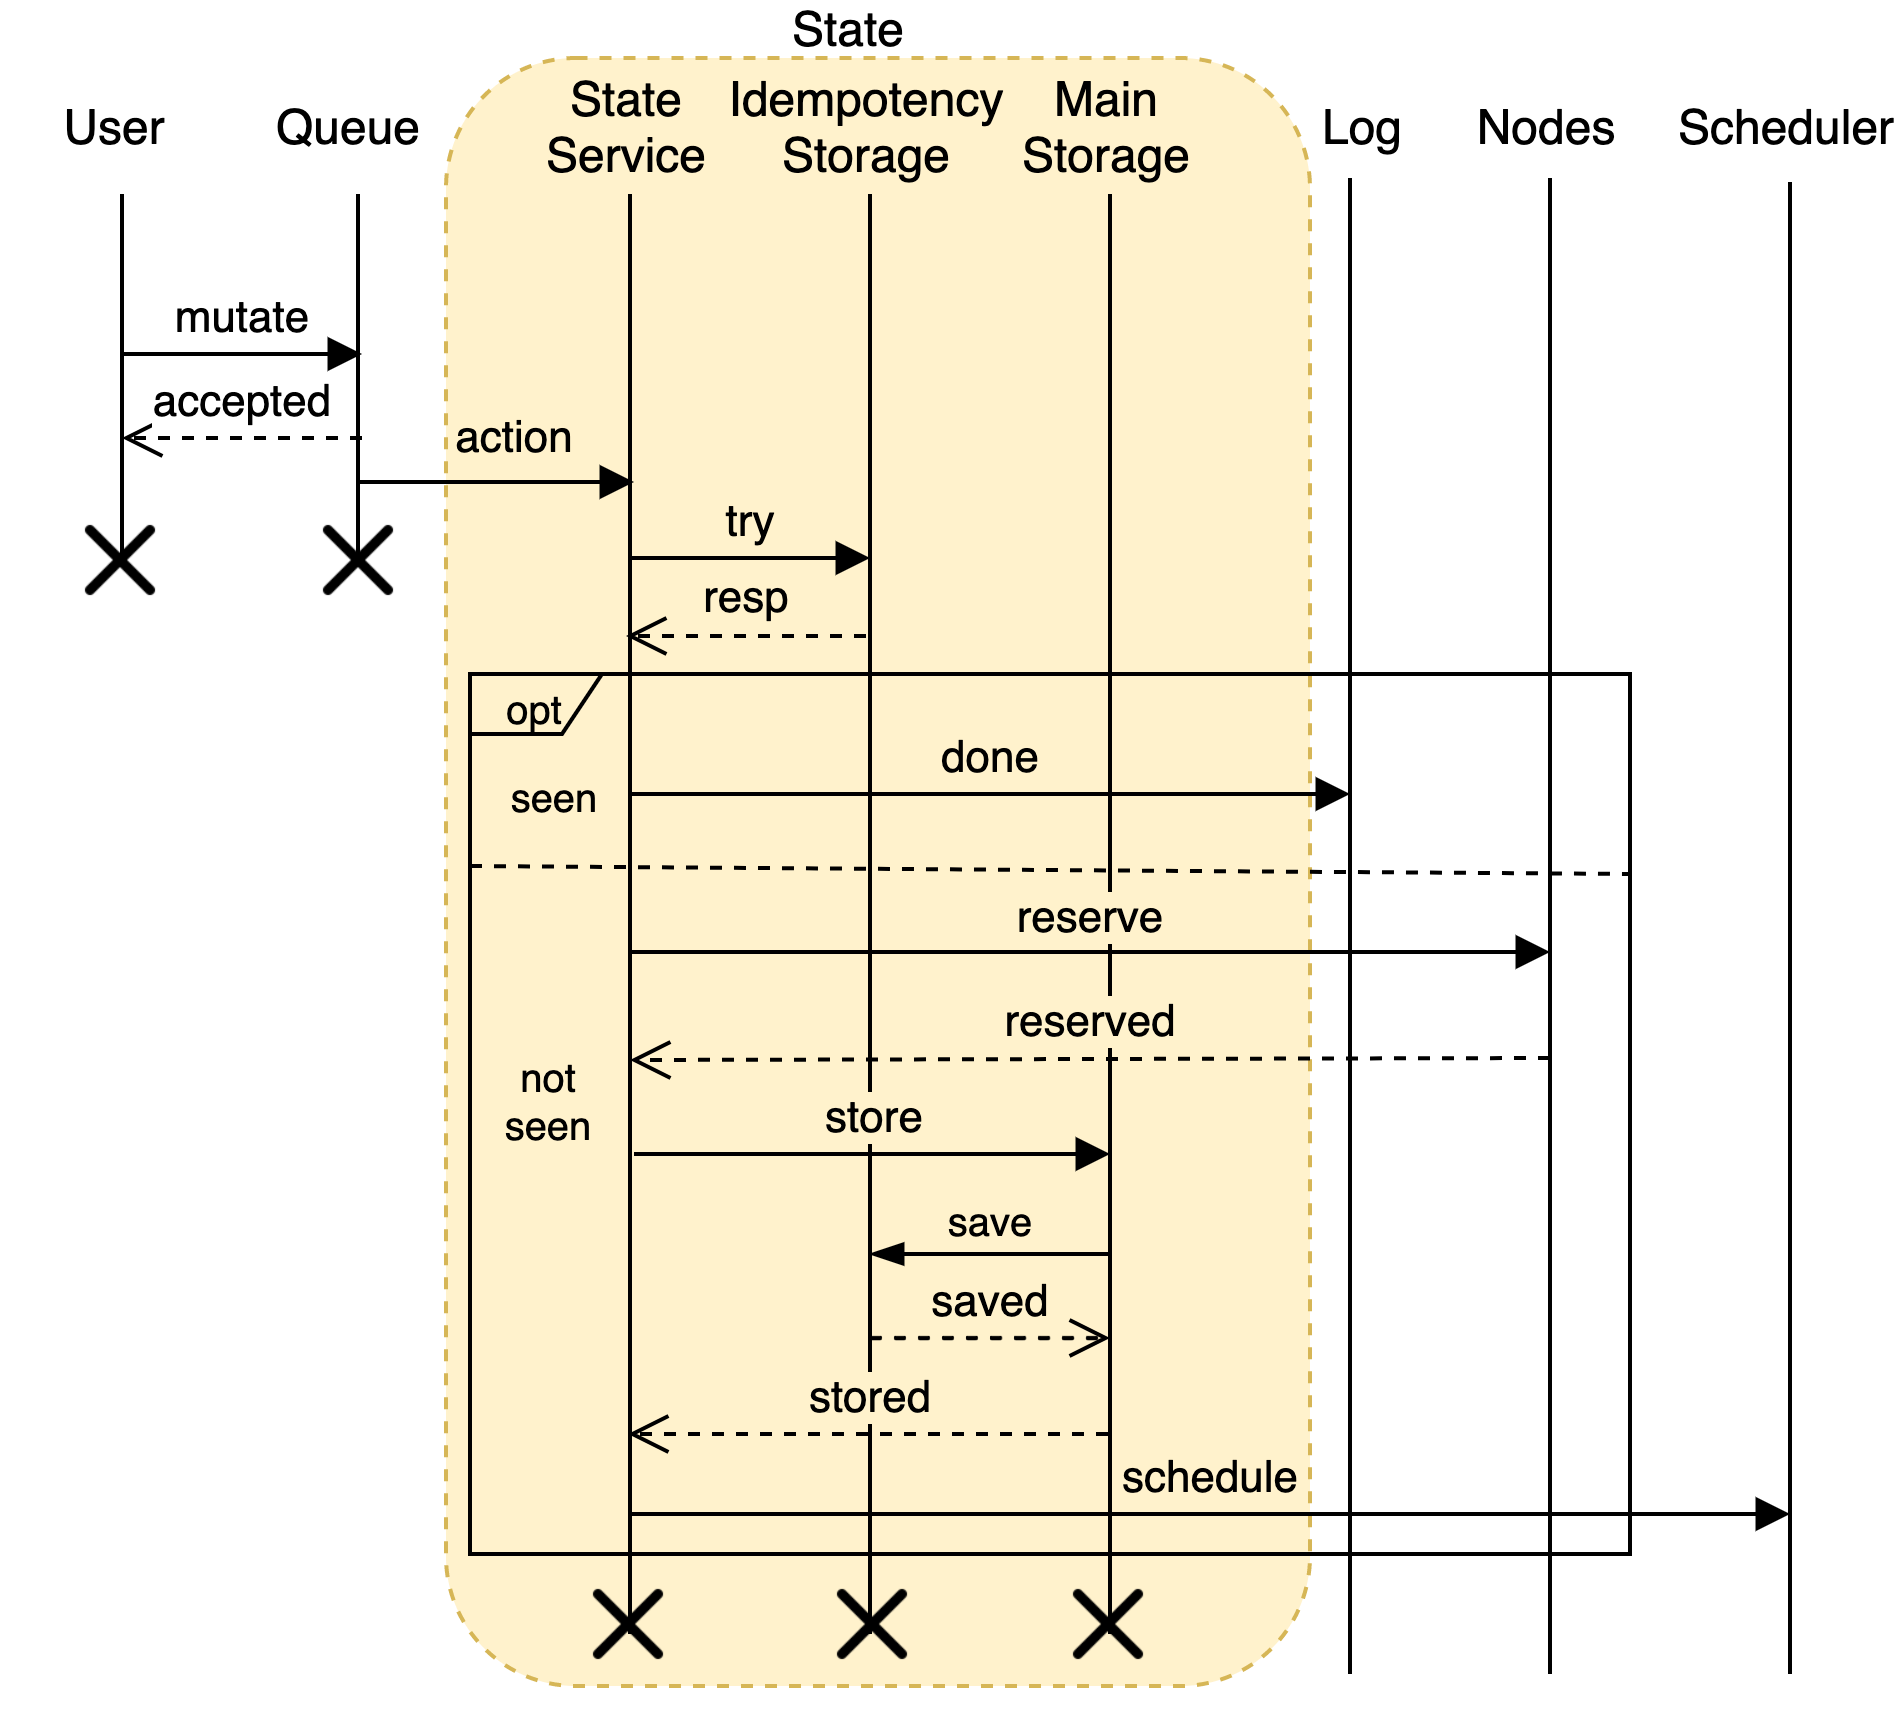
\includegraphics[scale=0.6]{images/Figure13}
	\end{center}
	\vspace{-0.7cm}
	\caption{Low level view of idempotency check communication.}
	\label{fig:fig13}
\end{figure}

\noindent
The participants follow the communication that we now describe informally: \label{informal_description_idempotency}

\begin{enumerate}[start=1,label={(\bfseries \arabic*)}]
	\item \textbf{User} sends a list request to State service (same as~\ref{sec:cluster_formation_protocol});
	\item \textbf{Queue} accepts the list request and the query local state based on the user selector. If a detailed view is required, the state gets metrics data from Nodes service (same as~\ref{sec:cluster_formation_protocol});
	\item \textbf{State service} is a wrapper aroud system main storage. Interacts with main storage in order to create new topologies, regions or clusters, or to get data from the main storages about the same entities. 
	\item \textbf{Idempotency storage} contains idempotent set for all \textbf{already} formed topologies, regions and clusters.
	\item \textbf{Main storage} contains records about the desired state for all formed topologies, regions, and clusters.
	\item \textbf{Log} contains records of operations. Users can query this service to see if their tasks are finished or have any problems (same as~\ref{sec:cluster_formation_protocol});
	\item \textbf{Nodes} accept messages from State. If possible, it will reserve desired nodes, otherwise, it will send an error message to Log service. On a health-check message, if a node is used in some cluster, it will inform that the node is alive (same as~\ref{sec:cluster_formation_protocol});
	\item \textbf{Scheduler} waits for a message sent from State, and pushes cluster formation messages to desired nodes (same as~\ref{sec:cluster_formation_protocol});
\end{enumerate}

\noindent
When testing idempotency, we must have in mind that stored structure could be: \textbf{(1)} flat keyspace, and \textbf{(2)} hierarchical keyspace. The both options are valid, as long as the \textbf{structure is idempotent}, and we can do \textbf{idempotent operations} over that structure. For example, $set$ as a data structure and $intersection$ are good candidates. It is worth noticing that the flat keyspace is a special case of the hierarchical keyspace.%For the purpose of this thesis, to bypass complex graph similarity algorithms, the hierarchical structure is translated into a flat keyspace structure, and the elements of that set are compared. %The algorithm that will test structure idempotency must be able to test both options. 
%For the future work, the algorithm should be designed in such a way that will be able to test structure idempotency must be able to test both options.
The algorithm that will test structure idempotency must be able to test both options.

Algorithm~\ref{alg:alg6} describes steps required to test if the operation is done before.

\begin{algorithm}[H]
	\SetKwFunction{equals}{equals}
	\SetKwProg{Fn}{function}{:}{}
	\tcp{children are sorted in both trees}
	\Fn{\equals{stored, topology}}{
		sChildren $\leftarrow$ stored.children\\
		tChildren $\leftarrow$ topology.children\\
		%\If{topology $==$ \textsc{null} $\lor$ topology.children.size $\neq$ stored.children.size $\lor$ stored.data $\neq$ topology.data}{
		\If{topology $==$ \textsc{null} $\lor$ tChildren.size $\neq$ sChildren.size \\ $\lor$ $\neg$ stored.isIdempotent(topology.data)}{
			\KwRet{false}
		}
	
		%sIter $\leftarrow$ sChildren.iterator\\
		%tIter $\leftarrow$ tChildren.iterator\\
		\While{sChildren.hasNext $\land$ tChildren.hasNext}{
			\If{$\neg$ equals(sChildren.next, tChildren.next)}{
				\KwRet{false}
			}
		}
		\KwRet{true}
	}
	
	\SetAlgoLined
	\SetKwInOut{Input}{input}
	\Input{request}
	stored $\leftarrow$ storage.findRequest(request.payload.name)\\
	\uIf{stored $\neq$ \textsc{null}}{
		\KwRet{false}
	}\Else{
		topology $\leftarrow$ request.payload.topology\\
		\KwRet{$\neg$ equals(stored, topology)}
	}
	\caption{Mutate idempotency check}
	\label{alg:alg6}
\end{algorithm}

\noindent
A formal description of the idempotency check protocol (see Figure~\ref{fig:fig13}) by using~\cite{HuY17} is presented next. The global protocol $\G_3$ (given below) conforms the informal description given at page~\pageref{informal_description_idempotency}. At this point, the $\mathtt{user}$ can choose one of two possible messages: 

\begin{enumerate}[start=1,label={(\bfseries \arabic*)}]
\item $\mathit{quit}$, in which case the protocol terminates; or, 
\item $\mathit{mutate}$, and the mutation process, described with global protocol $\G'$, starts;
\end{enumerate}
\begin{align*}
\G_3 & = 
\left\{
\begin{array}{@{}l@{}}  
\mathtt{user}\to\mathtt{service}{:} \mathit{quit}().\tend\\
\mathtt{user} \to \mathtt{service}{:}\mathit{create}(\T_3).
\mathtt{state} \to \mathtt{user}{:}\mathit{ok}().\G'
\end{array} \right.
\end{align*}
\myequations{Idempotency check global protocol.}

The mutate protocol $\G'$, activated in the first branch in $\G_3$, starts with $\mathtt{user}$ sending 
$\mathtt{create}$ message to $\mathtt{state}$, specifying also information about the new user desired state typed with $\T_3$, 
and $\mathtt{state}$ replies back with $\mathit{ok}$. This process is the same as cluster formation protocol (see Section~\ref{cluster_formation_informal_description}). Now we start specific communication protocol for idempotency check so $\mathtt{service}$ sends payload $T_3$ to $\mathtt{istorage}$ to test if this request is $seen$ before. The $\mathtt{istorage}$ responds with payload $T_6$ to $\mathtt{service}$, and based on $Boolean$ response $\mathtt{service}$ can do one of two things:

\begin{enumerate}[start=1,label={(\bfseries \arabic*)}]
	\item $\mathtt{service}$ sends message to $\mathtt{log}$ and this process terminates; or,
	\item $\mathtt{service}$ sends $\mathit{ids}$ of the nodes to be reserved (specified in the payload typed with $\T_4$) to $\mathtt{nodes}$;
\end{enumerate}

\noindent
same as cluster formation protocol (see Section~\ref{cluster_formation_informal_description}). For simplification, we can assume that all nodes are reserved, and now idempotency data store global protocol $\G''$, starts;
\begin{align*}
G' & = 
\mathtt{service} \twoheadrightarrow \mathtt{istorage}{:}\mathit{try}(\T_3). \\
& \hspace{1mm}
\mathtt{istorage} \to \mathtt{service}{:}\mathit{resp}(\mathsf{Boolean}).\\
& \hspace{10mm}
\left\{
\begin{array}{@{}l@{}}
\mathtt{service} \twoheadrightarrow\mathtt{log}{:} \mathit{done}(\mathsf{String}).\tend\\
\mathtt{service} \twoheadrightarrow\mathtt{nodes}{:}\mathit{ids}(\T_4).
\mathtt{nodes} \to \mathtt{service}{:}\mathit{rsrvd}().\G''
\end{array} \right.
\end{align*}

\noindent
The idempotency store protocol $\G''$, starts with $\mathtt{service}$ sending mutation payload $T_3$ to $\mathtt{mstorage}$. Then $\mathtt{mstorage}$ sends the same payload to $\mathtt{istorage}$. When data is saved for future testing, $\mathtt{istorage}$ responds back to $\mathtt{mstorage}$, and finally $\mathtt{mstorage}$ responds back to $\mathtt{service}$. At this point user payload $T_3$ is stored in both main storage and idempotency storage for future testing. Protocol continues with $\mathtt{state}$ connects $\mathtt{sched}$ (Scheduler) with message $\mathit{ids}$ and the payload that contains other data imported for mutation to be completed (typed with $\T_5$), and the rest of cluster formation protocol may continue.

\begin{align*}
\G'' = & 
\mathtt{service} \twoheadrightarrow \mathtt{mstorage}{:}\mathit{store}(\T_3).
\mathtt{mstorage} \twoheadrightarrow \mathtt{istorage}{:}\mathit{save}(\T_3).\\
& \hspace{4mm}
\mathtt{istorage} \to \mathtt{mstorage}{:}\mathit{saved}().
\mathtt{mstorage} \to \mathtt{service}{:}\mathit{stored}().\\
& \hspace{4mm}
\mathtt{service} \twoheadrightarrow \mathtt{sched}{:}\mathit{ids}(\T_5).\tend
\end{align*}

\noindent
We may now obtain the projections of global type $\G_3$ onto the participants $\mathtt{user}, \mathtt{service}, \mathtt{istorage}$, $\mathtt{mstorage}$, $\mathtt{log}$, $\mathtt{nodes}$: and $\mathtt{sched}$:

\begin{align*}
\ST_\mathsf{user} = &
{+}
\left\{
\begin{array}{@{}l@{}}
\mathtt{service}{!}\mathit{quit}().\tend\\
\mathtt{service}{!}\mathit{create}(\T_3).\mathtt{service}{?}\mathit{ok}().\tend\\
\end{array} \right.
\end{align*}
\begin{align*}
	\ST_\mathsf{service} = &
	{+}
	\left\{
	\begin{array}{@{}l@{}}
	\mathtt{user}{?}\mathit{quit}().\tend \\
	\mathtt{user}{?}\mathit{create}(\T_3).\mathtt{user}{!}\mathit{ok}().\ST'\\
	\end{array} \right.
\end{align*}
where
\begin{align*}
	\ST' = &
	\mathtt{istorage}{!!}\mathit{try}(\T_3).\mathtt{istorage}{?}\mathit{resp}(\mathsf{Boolean}).\\
	&
	{+}
	\left\{
	\begin{array}{@{}l@{}}
	\mathtt{log}{!!}\mathit{done}(\mathsf{String}).\tend\\
	\mathtt{nodes}{!!}\mathit{ids}(\T_4).\mathtt{nodes}{?}\mathit{rsrvd}().\ST''\\
	\end{array} \right.
\end{align*}
\begin{align*}
	\ST_\mathtt{mstorage} =  & \hspace{2mm}
	\mathtt{service}{??}\mathit{store}(\T_3).\mathtt{istorage}{!!}\mathit{save}(\T_3).\\ & \hspace{-8mm}
	\mathtt{istorage}{?}\mathit{saved}().\mathtt{service}{!}\mathit{stored}().\tend
\end{align*}
\begin{align*}
	\ST'' = & 
	\mathtt{mstorage}{!!}\mathit{store}(\T_3).\mathtt{mstorage}{?}\mathit{stored}().\\ & \hspace{-8mm}
	\mathtt{sched}{!!}\mathit{ids}(\T_5).\tend
	%\end{align*}
	%
	%\begin{align*}
\end{align*}
\begin{align*}
	\ST_\mathtt{istorage} =  &
	\mathtt{service}{??}\mathit{try}(\T_3).\mathtt{service}{!}\mathit{resp}(\mathsf{Boolean}).\\ & \hspace{-8mm}
	\mathtt{mstorage}{??}\mathit{save}(\T_3).\mathtt{mstorage}{!}\mathit{saved}().\tend
\end{align*}
\begin{align*}
	\ST_\mathtt{log} =  &
	\mathtt{service}{??}\mathit{done}(\mathsf{String}).\tend
\end{align*}
\begin{align*}
	\ST_\mathtt{nodes} =  &
	\mathtt{service}{??}\mathit{ids}(\T_4).\mathtt{service}{!}\mathit{rsrvd}().\tend
\end{align*}
\myequations{Idempotency check global protocol projection.}

\noindent
Similarly, as for $G_2$, we remark $\G_3$ could also be modeled using standard MPST (e.g.,~\cite{HondaYC08}), but again the projection types would be undefined while following the approach of ~\cite{HuY17} with explicit connections, all valid projections have been obtained.
%
%
\subsection{List detail protocol}\label{sec:list_detail_protocol}
%
The final communication protocol in our system appears in the information retrieval process. Using labels, the user can specify what part of the system he wants to retrieve, namely, on formed topologies. This protocol could be useful, for example, if the user wants to visualize his topologies, regions, or clusters on some dashboard and monitor for some changes, alerts, etc. 

This operation may span over multiple services to retreive complete informations about the clusters and/or nodes. For this purpose some of the distributed queries methods (see Section~\ref{sec:distributed_queries}) can be used. For some patterns api composition may be more suited, while for others CQRS may be the better solution to optimize queries.

This protocol comes with two available options: 

\begin{enumerate}[start=1,label={(\bfseries \arabic*)}]
	\item \textbf{global view} of the system -- all topologies the user manages. This will return just basic information about regions and clusters and their utilization;
	\item \textbf{specific clusters} details -- in-depth details for specified clusters like resources utilization over time (using stored metrics information), node information, configuration data, and running or stopped services.
\end{enumerate}

\noindent
It is important to note, that similarly to the query operation (defined previously), both rules $(\ref{eq:eq1})$ and $(\ref{eq:eq2})$ \textbf{must} be satisfied for information to be presented in the response. The user can specify one additional information in the list request, and that is whether or not the user wants a detailed view or not. If such information is presented in the request, the user will get a detaild view back. 

Figure~\ref{fig:fig8} shows a low-level view of the list operation protocol, where users can get details about the formed system. This setting involves the next participants: User, State, Nodes, and Log. 

\begin{figure}[!htbp]
	\begin{center}
		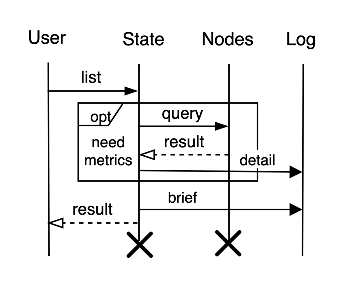
\includegraphics[scale=0.9]{images/FIG4}
	\end{center}
	\vspace{-0.4cm}
	\caption{Low level view of list operation communication.}
	\label{fig:fig8}
\end{figure}

\noindent
Now we can informally describe the roles of the participants in the protocol:\label{list_protocol_informal_description}, shown in figure~\ref{fig:fig8}

\begin{enumerate}[start=1,label={(\bfseries \arabic*)}]
	\item \textbf{User} sends a list request to State;
	\item \textbf{State} accepts the list request and the query local state based on the user selector. If a detailed view is requested, the state gets metrics data from Nodes, and return details back to user;
	\item \textbf{Nodes} contain node metrics data, and if required, it may send this data to State;
	\item \textbf{Log} contains records of all operations. Users can query this service.
\end{enumerate}

\noindent
Algorithm~\ref{alg:alg5} describes steps that are required after the state receives a list message.

\begin{algorithm}[H]
	\SetAlgoLined
	\SetKwInOut{Input}{input}
	\Input{request}
	Initialize: data $\leftarrow$ []\\
	\ForEach{(topology, isDetail) $\in$ userData(request.query)}{
		\uIf{isDetail}{
			data.append(topology.collectData())\\
		}\Else{
			data.append(topology.data())\\
		}
	}
	\Return data
	\caption{List of current state of the system}
	\label{alg:alg5}
\end{algorithm}

\noindent
A formal description of the list communication protocol (see Figure \ref{fig:fig4}) by using~\cite{HuY17} is presented next. Global type $\G_4$ (given below) starts with $\mathtt{user}$ connecting $\mathtt{state}$ with one of the two possible messages: 
\textbf{(1)} $\mathit{list}$, specifying a request for a detailed view, where sort $\T_1$ identifies which parts of the system the user wants to view in details, after which $\mathtt{state}$ connects $\mathtt{nodes}$ with $\mathit{query}$ message, with a payload of sort $\T_2$  containing specification of which nodes need to show their metrics data, and then protocol proceeds as prescribed with $\G'$; 
\textbf{(2)} $\mathit{list^*}$, specifies no need for a detailed view is specified, where a payload of sort $\T_4$ denotes user specified parts of the system the user wants to view, but without greater details. In the latter case protocol follows global type $\G''$.
\begin{align*}
\G_4 &= 
\left\{
\begin{array}{@{}l@{}}  
\mathtt{user} \twoheadrightarrow \mathtt{state}{:}\mathit{list}(\T_1).\mathtt{state}\twoheadrightarrow\mathtt{nodes}{:}\mathit{query}(\T_2). \G' \\
\mathtt{user} \twoheadrightarrow \mathtt{state}{:}\mathit{list^*}(\T_4).\G''
\end{array} \right.
\end{align*}
\myequations{List detail global protocol.}
Global type $\G'$ starts with $\mathtt{nodes}$ replying to $\mathtt{state}$ $\mathit{result}$ message and a payload identifying parts of the system user wants to see in greater detail typed with $\T_3$. Then, $\mathtt{state}$ connects $\mathtt{log}$ with $\mathtt{details}$ and also sends $\mathtt{result}$ to $\mathtt{user}$, and finally terminates. 
In $\G''$, $\mathtt{state}$ also connects $\mathtt{log}$ with $\mathit{brief}$ and a payload typed with $\T_5$ identifying parts of the system the user wants to see without greater detail. Then, $\mathtt{state}$ replies to $\mathtt{user}$ with $\mathtt{result}$ message, and the protocol terminates.
\begin{align*}
\begin{split}
	\G' =  & 
	\mathtt{nodes}\to\mathtt{state}{:}\mathit{result}(\T_3).\mathtt{state}\twoheadrightarrow \mathtt{log}{:}\mathit{detail}(\T_3). \\
	& \hspace{2mm}
	\mathtt{state}\to\mathtt{user}{:}\mathit{result}(\T_3).\tend
\end{split}
\end{align*}
\begin{align*}
	\G'' = &
	\mathtt{state}\twoheadrightarrow \mathtt{log}{:}\mathit{brief}(\T_5).\mathtt{state}\to\mathtt{user}{:}\mathit{result}(\T_5).\tend
\end{align*}

\noindent
Same as for the health-check and the cluster formation protocols, here we also present the projections of global type $\G_4$, modeling the list protocol, onto participants $\mathtt{user}$, $\mathtt{state}$, $\mathtt{nodes}$, and $\mathtt{log}$:
\begin{align*}
	\ST_\mathtt{user} =& 
	{+}
	\left\{
	\begin{array}{@{}l@{}}  
	\mathtt{state}{!!}\mathit{list}(\T_1).\mathtt{state}{?}\mathit{result}(\T_3).\tend \\
	\mathtt{state}{!!}\mathit{list^*}(\T_4).\mathtt{state}{?}\mathit{result}(\T_5).\tend 
	\end{array} \right.
\end{align*}
\begin{align*}
	\ST_\mathtt{state} =&
	{+}
	\left\{
	\begin{array}{@{}l@{}}  
	\mathtt{user}{??}\mathit{list}(\T_1).\mathtt{nodes}{!!}\mathit{query}(\T_2).\ST'\\
	\mathtt{user}{??}\mathit{list^*}(\T_4).\mathtt{log}{!!}\mathit{brief}(\T_5).\mathtt{user}{!}\mathit{result}(\T_5).\tend
	\end{array} \right. 
\end{align*}
where
\begin{align*}
	\ST'  =& 
	\mathtt{nodes}{?}\mathit{result}(\T_3).\mathtt{log}{!!}\mathit{detail}(\T_3).\mathtt{user}{!}\mathit{result}(\T_3).\tend
\end{align*}
\begin{align*}
	\ST_\mathtt{nodes} = &
	\mathtt{state}{??}\mathit{query}(\T_2).\mathtt{state}{!}\mathit{result}(\T_3).\tend
\end{align*}
\begin{align*}
	\ST_\mathtt{log} = & 
	{+}
	\left\{
	\begin{array}{@{}l@{}}  
	\mathtt{state}{??}\mathit{detail}(\T_3).\tend \\
	\mathtt{state}{??}\mathit{brief}(\T_5).\tend \\
	\end{array} \right.
\end{align*}
\myequations{List detail global protocol projection.}

\noindent
For instance, type $\ST_\mathtt{log}$ specifies $\mathtt{log}$ gets included in the session only after receiving from $\mathtt{state}$, either message $\mathit{detail}$, or message $\mathit{brief}$, and then terminates. 

Similarly as for $\G_2$ and $\G_3$ we remark $\G_4$ could also be modeled using standard MPST (e.g.,~\cite{HondaYC08}), but again the projection types would be undefined, while following the approach of ~\cite{HuY17} with explicit connections, all valid projections have been obtained.
%
%
\section{Long-lived transactions in micro clouds}\label{sec:long_live_transactions}
%
To operate $\upmu$Cs properly, such a system needs to be scalable. Architecture composed of loosely coupled services can be a way to go, because of all benefits such systems offer (see Section~\ref{sec:microservices}). But still, we must be aware of all problems that come along with them.

That being said, one of the problems we have to deal with are transactions that appear in such distributed system --- distributed transactions (see Section~\ref{sec:distributed_transactions}). Because of the nature of the system \emph{sagas} seems like a better pattern to use (see Section~\ref{sec:sagas}).

When a user submits new \emph{cluster creation message} (see Section~\ref{sec:cluster_formation_protocol}), the message will be accepted by the system, and the new task with \emph{PENDING} state will be registered. If for whatever reason (e.g., no available resources or nodes, etc.), the system cannot proceed further, that task is terminated. It goes to \emph{FAILED} state, concluding the transaction. Otherwise, no errors occured, and the system can proceed with the cluster formation protocol, changing the task state to \emph{IN PROGRESS}.

In this state, the system needs to do several things: \textbf{(1)} save newly formed cluster information, \textbf{(2)} prepare metrics service, \textbf{(3)} add watchers for the cluster nodes health-check, etc. This spans multiple services, creating a few sub-transactions in the process. The \emph{task state} prevents the users to apply other tasks (e.g., configurations, actions, autoscaling, etc.) on a not yet fully formed cluster.

Separation on sub-transactions allow us to invoke the rollback mechanism, if the process yields any errors. Other strategy would be to start some of the retry strategies in order to fix the occurred issue.

If no errors occur during the process, the \emph{cluster formation transaction} finishes, and the task state is changed to \emph{CREATED}. Otherwise, the \emph{cluster formation transaction} ends, \emph{without creating the cluster}. The task state will be changed to \emph{FAILED} state, concluding the transaction.

Figure~\ref{fig:fig19} shows state diagram for cluster formation message.

\begin{figure}[H]
	\begin{center}
		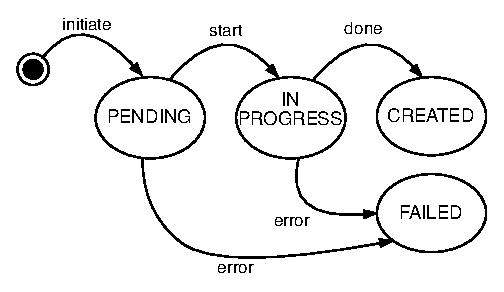
\includegraphics[scale=1]{images/Figure19}
	\end{center}
	\vspace{-0.6cm}
	\caption{State diagram for cluster formation message}
	\label{fig:fig19}
\end{figure}

Cluster formation protocol will most likely span over multiple services, and strategies like sagas can be useful to implement transactions and rollbacks properly.
%
%
\subsection{Garbage collection in micro clouds}\label{sec:garbage}
%
When the user submits the task to the system, and if, for whatever reason that task fails, there is the option to immediately remove that task, and possibly all task connected items. Or, the system should have a specific process in the background, which only purpose is garbage collection to restore unused and fragmented system resources.

The second option seems more acceptable because one item can have a graph of items that are connected to that specific item. This graph can be complex, and immediate deletion may slow down the entire system. In the background, the garbage collection process can mark unused items and delete them when the time is right.

Users should also be able to delete certain items with their dependencies as well, invoking \emph{cascading deletion}. Dependencies may be deleted immediately, or marked as \emph{orphans}, and deleted by the garbage collection process.

It makes sense that users can influence garbage collection by submitting their policies when and how often to do this operation, to delete only items or container images as well, and so on.
%
%
\section{System observability}\label{sec:system_observability}
%
Observability is an importatnt part of any real-world computing system (see page~\pageref{sec:log_aggregation}). It is an important part of any platform that strives to be offered as a service to large groups of different users. 

At every moment, we must know what is happening in the system, where bottlenecks are, and how we can resolve problems. This is of significant importance in DS, where state and calculations are scattered across multiple nodes, clusters and even DCs.

In the $\upmu$Cs environment that involves multiple layers (see page~\pageref{lab:three-tier}), this technique is even more important to give us insight what is happening in the system, and how we can optimize different layers of the system. On the other hand, users who use such a system need to know what is happening with their services.

Because of these two really important parameters, observability must be implemented on two levels:

\begin{enumerate}[start=1,label={(\bfseries \arabic*)}]
	\item \textbf{System level} contains data that is generated by the system. This data should be avalible to the administrators and providers of the system \textbf{only}. Operations people in the team (eg. DevOps or SREs), and developers cannot see it;
	\item \textbf{User level} contains information about user requests that \textbf{only} operations people in the team (eg. DevOps or SREs) should be able see it. This type of data should not be visible to the system providers, for privacy reasons.
\end{enumerate}

\noindent
Every service should log details about its usage and calls as well as traces how requests are going, regardless of whether it is a platform or user. Log data should be stored outside the service and the virtualization tool (eg. using sidecar pattern with containers~\cite{BurnsO16}), while pieces of information will be sent to centralized log storage. Sending intervals should be able to be changed and adapted for both levels.

Log storage could be searched to see the general state of the system, and pieces of information about user requests and the state of their requests.
%
%
\section{Access pattern}\label{sec:access_pattern}
%
In section~\ref{sec:application_model}, we already discussed system access patterns from the applications point of view, using streams and topics. In this section, we are going to venture into the dashboard and system access described in~\ref{sec:distribution_models}. 

To access the system, requests are going over the \textit{master process}. This process is not responsible for any sort of synchronization, agreement, or something like that, but just to show dashboards and various system details since the cloud is available anywhere in the world, while $\upmu$C should serve the local population. 

One question that could come to mind is, what if some cloud provider offering $\upmu$C functionality, or running our master process, goes down, should the rest of the $\upmu$Cs go to \textit{read-only} mode and only accept \textbf{read} requests?

All communication is not exclusive to go over that master process, but if the user is nearby to $\upmu$C he/she should be able to initiate commands directly to clusters, regions, and topologies. However, for dashboards and full pieces of information about his $\upmu$Cs, cloud would be a better solution, because of more available resources.

If some cloud provider goes down for whatever reason, we should foresee this, and to resolve it, we could use multiple cloud providers using \textit{Multi-Cloud Computing}~\cite{HongDSH19, Ardagna15} so that one cloud provider is a master process and many others are backup in case the whole cloud provider goes down.

We inevitably have some state synchronization here, and we could rely on SEC and CRDTs to do synchronization without some expensive coordination between providers.

This is not generally a problem if applications that are running in $\upmu$Cs are not dependent on some process, location, sensors of services, etc. If this is the case, then we can connect $\upmu$Cs in sort of \emph{P2P network} and give them some logic to just route request to the proper location on the globe. 

This might not be that fast, since even light is affected by the distance, but we would be able to issue requests to cluster in a different part of the world.
%
%
\section{Auto scaling micro clouds}\label{sec:Auto Scaling}
%
Configurable model structure bring any additional benefit to proposed $\upmu$Cs model --- infrastructure \textbf{auto scaling}. 

The purpose of this process is to automatically scale up or down existing clusters, regions even topologies, adapting the number of nodes in the cluster, clusters per region, and even regions per topology to match newly workload increase.

The users can create a scaling plan via scaling policies, where they should be able to define: \textbf{(1)} how resources should be added (e.g., grow clusters, regions, or topologies) and at which rate, \textbf{(2)} what specific type of resources are desired (e.g., prefered values for CPU, disk, memory etc.), and \textbf{(3)} boundaries for both resource additions and resource types.

The third item is increasingly important, because it directly affect the costs of the applications running inside $\upmu$Cs. As such, it should never be underlooked.

Based on the given policies the autoscaler dynamically adjusts the amount of resources according to user demands~\cite{TamiruTEP20}. This elasticity allows accommodation of fluctuations in the workloads, that vary over time.

Auto scaling strategy could be applied to both applications and infrastructure, and $\upmu$C provider should decide should they depend on each other, or should they be regulated separately. The proposed model could accomodate both options.
%
%
\section{User data flow in micro clouds}\label{sec:user_data}
%
One of the benefits of having $\upmu$C in near proximity is that user data can be processed and stored locally, and users are able to control to which extent data can be shared with the cloud~\cite{SatyanarayananK19} (see section~\ref{sec:problem_statement}). 

User data would be relatively easy to replicate inside a region using CRDTs for example (see~\ref{crdts}), to eliminate expensive coordination~\cite{inproceedingsSimic2}. On top of this, distributed file system can be built, distributed databases, processing frameworks specially designed for $\upmu$C environment.

But since $\upmu$Cs storage capacity is less than traditional cloud, they should store most recently used data~\cite{SimicSensors}. The storage capacity is determined by the $\upmu$C size given by the equation~\ref{size:eq1}.

\textbf{Data locality} in $\upmu$Cs creates two challenges, that must be addressed:

\begin{enumerate}[start=1,label={(\bfseries \arabic*)}]
	\item A user leaves a place, is data stationary, or follows him using some pattern? The decision should be left to users, $\upmu$C providers, and developers to decide. The proposed model allows the creation of different \textbf{data plans} that could be represented via \textbf{different policies} for every individual user or group of users. If data needs to follow the user, as a data transfer medium the cloud could be used as a backbone, to transfer data to the $\upmu$C in user proximity. The process is similar to the content delivery networks on the edge~\cite{inbookKurniawan}. In such a scenario, we must pay attention to the network pressure and transfer only the requested data. As an alternative option, we can serve data directly from the cloud and do not transfer anything;
	\item How long the user data should be stored in the $\upmu$C, if we assume that locally existing $\upmu$C will serve many users? The proposed model does not restrict how long the data should be stored and it is \textbf{policy-based}. Depending on the $\upmu$C size given by equation~\ref{size:eq1}, $\upmu$C providers may determine \textbf{different policies} --- Time to live (TTL)~\cite{CohenHK05} and offer to users. This process is somewhat similar to the leases mechanism in cache systems~\cite{GrayC89}. 
\end{enumerate}

The data retention and size in the $\upmu$C are decided and optimized with~\ref{size:eq1} and~\ref{size:eq2}, for the single user or group of users. This gives developers, and $\upmu$C providers more room to optimize their policies offered to the users, while users may choose different options based on their needs~\cite{SimicSensors}.
%
%
\section{Extendability}\label{sec:extendability}
%
The proposed system allow extension, and could be used for addition of various configurations and artifacts to \emph{nodes, clusters, regions} and even \emph{topologies} --- $\upmu$Cs, all done remotely. 

As the direct implication of \emph{reconcile pattern} (see page~\pageref{loop_pattenr}), extension is as easy as adding the new worker to the system. This new worker, will deal with a specific resource type when that kind of file is submitted to the system.

On the other hand, a \emph{reconcile loop} (see page~\pageref{reconcile_loop}) will provide the observed resource informations that this worker can act on. This mean that specific worker (controller) will deal with just one resouce type at any given point in time knowing what is specified, and what is returned from reconcile loop. 

When registering new worker, a user should provide \emph{unique} name of the worker so that reconcile loop can send informations to the right place. As a unique name we can use for examle worker name and resource type name.

Figure~\ref{fig:fig30} show high overview of adding a new worker to the system, with reconcile loop.

\begin{figure}[H]
	\begin{center}
		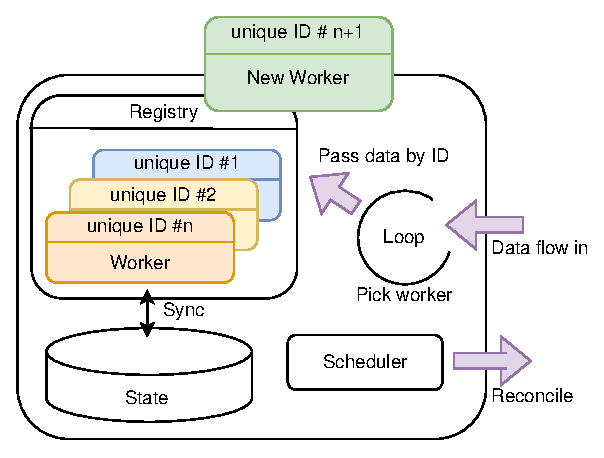
\includegraphics[scale=0.7]{images/Figure30}
	\end{center}
	\vspace{-0.7cm}
	\caption{New worker addition to the system, with reconcile loop.}
	\label{fig:fig30}
\end{figure}
%
%
\section{Repercussion}\label{sec:repercussion}
%
The model presented in this chapter, has four possible model repercussions:

\begin{enumerate}[start=1,label={(\bfseries \arabic*)}]
	\item \textbf{Stand alone}, the proposed model can serve as a base layer for future ECC as a service implementation. On top of it, we can implement other services and features like scheduling, storage, applications, management, monitoring, etc. As such it could be a viable option in the CC;
	\item \textbf{Integration}, the proposed model could be integrated with existing systems like Kubernetes, OpenShift, or cloud provider infrastructure since they all operate over the cluster. This is possible, with some small infrastructure changes and adaptations because -- the communication should be implemented via standard interfaces like HTTP and JSON, the integrations should be relatively easy to achieve. The proposed model could be used as a geo-distributed description and/or an organization tool;
	\item \textbf{Combination}, this approach can be done over multi-cloud principles. Some cloud tasks could be offloaded to the nearest $\upmu$C;
	\item \textbf{Enhancement}, big data tools, esspecially lambda architecture (see Section~\ref{sec:big_data}) could be enhanced using the proposed model creating \textbf{lambda++} architecture. Here we can reduce cost even more, by doing preprocessing and filtering of data closer to their source. After that we can send processed data to stream processing part of traitional lambda architecture, allowing it to process even more data than before.
\end{enumerate} 
%
%